\documentclass[10pt, a4paper]{article}

% Parametri che modificano il file main.tex
% Le uniche parti da cambiare su main.tex sono:
% - vari \vspace tra sezioni
% - tabella azioni da intraprendere
% - sezione altro

\def\data{2024-03-12}
\def\oraInizio{14:00}
\def\oraFine{15:30}
\def\luogo{Piattaforma Discord}

\def\tipoVerb{Interno} % Interno - Esterno

\def\nomeResp{Orlandi G.} % Cognome N.
\def\nomeVer{Bresolin G.} % Cognome N.
\def\nomeSegr{Michelon R.} % Cognome N.

\def\nomeAzienda{Azzurro Digitale}
\def\firmaAzienda{azzurrodigitale.png}
\def\firmaResp{giacomo.png} % nome Responsabile

\def\listaPartInt{
Bresolin G.,
Campese M.,
Ciriolo I.,
Dugo A.,
Feltrin E.,
Michelon R.,
Orlandi G.
}

\def\listaPartEst{
Azzurro B.,
Digitale C.,
}

% Se nessuna revisione: \def\listaRevisioneAzioni {x}
\def\listaRevisioneAzioni {x}

\def\listaOrdineGiorno {
{Aggiornamento da parte di tutti i membri del gruppo riguardo al lavoro di codifica iniziato dopo la riunione precedente;},
{Preparazione per la riunione con l'azienda pianificata in data 2024-03-13;},
{Assegnazione dei task relativi alla parte di testing.}
}

\def\listaDiscussioneInterna {
{Il team ha eseguito un aggiornamento generale relativo alla codifica del backend in corso da una settimana. Considerati i buoni risultati il gruppo ha discusso della possibilità di presentare il lavoro svolto durante la riunione con AzzurroDigitale pianificata per il 2024-03-13;},
{Il team ha riportato la discussione tenuta in settimana per la divisione del lavoro da svolgere riguardante la parte di test di unità delle componenti sviluppate durante la prima parte di codifica del progetto. La suddivisione delle task viene quindi riportata in 'Azioni da intraprendere'.
}
}



% Se nessuna decisione: \def\listaDecisioni {x}
\def\listaDecisioni{
{Il team presenterà all'azienda il lavoro di codifica delle componenti di backend svolto fino ad ora;},
{Il team continuerà la produzione della parte di test di unità delle componenti di backend secondo la suddivisione dei compiti riportata in 'Azioni da intraprendere'.}
}

\usepackage{style}
\usepackage{headerfooter}

\title{\titolo}
\author{SWEetCode}

\begin{document}

% PRIMA PAGINA
\begin{titlepage}
    \thispagestyle{empty}
    \begin{tikzpicture}[remember picture, overlay]
        % TRIANGOLI
        \draw[fill=secondarycolor, secondarycolor] (current page.north west) -- (current page.south west) -- (8.8, -28);
        \draw[fill=primarycolor, primarycolor] (-3, 5) -- (4, -13.6) -- (11, 5);

        % LOGO
        \node [xshift=-5cm, yshift=25cm] (logo) at (current page.south east) {
\includegraphics[width=6.5cm]{img/logo.png}};

        % SWEETCODE - DATE
        \node [anchor=north east, align=right, xshift=-1.2cm, yshift=20.5cm, text=black] (sweetcode) at (current page.south east) {\fontsize{32pt}{36pt}\selectfont SWEetCode};
        \draw[line width=4pt, lightcol] ([xshift=-3cm, yshift=-0.37cm]sweetcode.south west) -- ([yshift=-0.37cm]sweetcode.south east);
        \node [anchor=north east, align=right, xshift=-1.2cm, yshift=18.7cm, text=black] (date) at (current page.south east){\fontsize{24pt}{24pt} \selectfont Verbale \tipoVerb};

        % NOME FILE
        \node [anchor=north east, text width=15cm, align=right, xshift=-1.2cm, yshift=17cm, text=black] (titolo) at (current page.south east){\fontsize{48pt}{48pt}\textbf{\data}};

        % BOX DATI PARTECIPANTI
        \ifthenelse{\equal{\tipoVerb}{Esterno}}{
            \node[anchor=north east, xshift=-1.2cm, yshift=14.5cm, minimum width=8cm] (box) at (current page.south east){};
        }{
            \node[anchor=north east, xshift=-1.2cm, yshift=12.5cm, minimum width=8cm] (box) at (current page.south east){};
        }

        % RESPONSABILE
        \node[anchor=north west, align=left] (dati2) at (box.north west) {\fontsize{15pt}{15pt}\selectfont \textbf{Responsabile}};
        \draw[line width=4pt, lightcol] (dati2.south west) -- ([xshift=8cm]dati2.south west);
        \node[anchor=north west, align=left] (dati21) at (dati2.south west){\fontsize{13pt}{13pt}\selectfont \nomeResp};

        % VERIFICATORE
        \node[anchor=north west, yshift=-1cm, align=left] (dati3) at (dati21.north west) {\fontsize{15pt}{15pt}\selectfont \textbf{Verificatore}};
        \draw[line width=4pt, lightcol] (dati3.south west) -- ([xshift=8cm]dati3.south west);
        \node[anchor=north west, align=left] (dati31) at (dati3.south west){\fontsize{13pt}{13pt}\selectfont \nomeVer};

        % SEGRETARIO DI RIUNIONE
        \node[anchor=north west, yshift=-1cm, align=left] (dati4) at (dati31.north west) {\fontsize{15pt}{15pt}\selectfont \textbf{Segretario di Riunione}};
        \draw[line width=4pt, lightcol] (dati4.south west) -- ([xshift=8cm]dati4.south west);
        \node[anchor=north west, align=left] (dati41) at (dati4.south west){\fontsize{13pt}{13pt}\selectfont \nomeSegr};
        
        % UNIPD - SWE
        \node [xshift=4.4cm, yshift=2.3cm, draw, secondarycolor, text=white] (uni) at (current page.south west) {\fontsize{20pt}{20pt} \selectfont Università di Padova};
        \node [xshift=0.65cm, yshift=0.7cm, draw, secondarycolor, text=white, below=of uni] (corso) {\fontsize{20pt}{20pt}\selectfont Ingegneria del Software};

        % FIRMA AZIENDA
        %\ifthenelse{\equal{\tipoVerb}{Esterno}}{
           % \draw[line width=4pt, lightcol] ([xshift=-1.2cm, yshift=5.2cm]current page.south east) -- ([xshift=-8cm, yshift=5.2cm]current page.south east);
          %  \node [xshift=-4.8cm, yshift=6.3cm] (logo) at (current page.south east) {\includegraphics[width=6cm]{img/firme/\firmaAzienda}};
          %  \node[anchor=north west, xshift=12.9cm, yshift=4.95cm, align=left] at (current page.south west)
           % {\fontsize{13pt}{13pt}\selectfont L'azienda: \nomeAzienda};
       % }

       %  FIRMA
        \draw[line width=4pt, lightcol] ([xshift=-1.2cm, yshift=1.8cm]current page.south east) -- ([xshift=-8cm, yshift=1.8cm]current page.south east);
        \node [xshift=-4.8cm, yshift=2.45cm] (logo) at (current page.south east) {\includegraphics[width=6cm]{img/firme/\firmaResp}};
        \node[anchor=north west, xshift=12.9cm, yshift=1.45cm, align=left] at (current page.south west)
        {\fontsize{13pt}{13pt}\selectfont Il Responsabile: \nomeResp};
        
    \end{tikzpicture}
\end{titlepage}

% REGISTRO DELLE VERSIONI
%Registro in ordine dalla più recente alla meno recente!

{\renewcommand{\arraystretch}{1.5}
\section*{Registro delle versioni}

\begin{xltabular}{\textwidth}{c|c|c|c|X}
\label{tab:long}

\textbf{Versione} & \textbf{Data} & \quantities{\textbf{Responsabile di}\\\textbf{stesura}}& \textbf{Revisore} & \quantities{\textbf{Dettaglio e}\\\textbf{motivazioni}} \\
\endfirsthead

\textbf{Versione} & \textbf{Data} & \quantities{\textbf{Responsabile di}\\\textbf{stesura}}& \textbf{Revisore} & \quantities{\textbf{Dettaglio e}\\\textbf{motivazioni}} \\
\endhead

\multicolumn{5}{r}{{Continua nella pagina successiva}} \\
\endfoot

\endlastfoot

\hline
v2.23.0(1) & $2024-03-20$ & \quantities{Ciriolo I.} & Feltrin E. & Gestione e visualizzazione delle chat.\\
\hline
v2.21.0(1) & $2024-03-19$ & \quantities{Ciriolo I.} & Michelon R. & Prima stesura.\\
\hline
    
\end{xltabular}}
\newpage

% INDICE
\tableofcontents
\newpage

% INTRODUZIONE
\section{Introduzione}
\subsection{Scopo del documento}
Il documento ha lo scopo di definire i casi d'uso della \textit{web application} che verrà sviluppata nel corso del progetto. Vengono inoltre presentati i requisiti funzionali, di qualità e di vincolo. %e le funzionalità aggiuntive che saranno implementate non essendo ritenute essenziali/necessarie.
\\
%\subsection{Scopo del prodotto}
\subsection{Glossario}
%\paragraph{}Per evitare ambiguità e incomprensioni relative al linguaggio e ai termini utilizzati nella documentazione relativa al progetto viene presentato un Glossario. I termini ambigui o specifici presenti nello stesso, verranno identificati con un pedice |g|. (DA VALUTARE COME RICONOSCERE IL TERMINE )

\subsection{Riferimenti}
   \subsubsection{Riferimenti normativi}
   \begin{itemize}
    \item \textit{Regolamento del progetto didattico}: \\
    \href{https://www.math.unipd.it/~tullio/IS-1/2023/Dispense/PD2.pdf}{https://www.math.unipd.it/\textasciitilde tullio/IS-1/2023/Dispense/PD2.pdf};
    \item \textit{\S Norme di progetto}.
    \end{itemize}
    
    \subsubsection{Riferimenti informativi}
    
    \begin{itemize}
   % \item \textit{Glossario v0.0.1} (da creare parallelamente); 
    \item \textit{Presentazione capitolato C1}:\\
    \href{https://www.math.unipd.it/~tullio/IS-1/2023/Progetto/C1.pdf}{https://www.math.unipd.it/\textasciitilde tullio/IS-1/2023/Progetto/C1.pdf};
    \item \textit{Verbali esterni ed interni};
    \item \textit{Analisi e descrizione delle funzionalità: Use Case e relativi diagrammi (UML):}\\
    \href{https://www.math.unipd.it/~rcardin/swea/2022/Diagrammi%20Use%20Case.pdf}{https://www.math.unipd.it/\textasciitilde rcardin/swea/2022/Diagrammi\%20Use\%20Case.pdf ;}
    \item \textit{Analisi e descrizione delle funzionalità: Diagrammi delle Attività (UML):}\\
    \href{https://www.math.unipd.it/~rcardin/swea/2022/Diagrammi%20di%20Attivit%C3%A0.pdf}{https://www.math.unipd.it/\textasciitilde rcardin/swea/2022/Diagrammi\%20di\%20Attivit\%C3\%A0.pdf;}
    

    \item \textit{Progettazione e Programmazione: Diagrammi delle Classi:}\\
    \href{https://www.math.unipd.it/~rcardin/swea/2023/Diagrammi%20delle%20Classi.pdf}{https://www.math.unipd.it/\textasciitilde rcardin/swea/2023/Diagrammi\%20delle\%20Classi.pdf.}
    \end{itemize}

% DESCRIZIONE
\newpage
\section{Descrizione}
\subsection{Obiettivi del prodotto}
Il proponente richiede la creazione di un sito web dotato di un chatbot realizzato tramite interrogazioni ad un modello di intelligenza artificiale, che sia d'aiuto a tutto il personale dell'azienda.
In particolare il sistema deve facilitare l'accesso dei dipendenti alle informazioni, regolamentazioni e alle indicazioni aziendali.\\
Il prodotto deve fornire nuove modalità di formazione e assistenza sul lavoro, superando i limiti di un classico \textit{repository} documentale, in maniera tale da rendere le informazioni più fruibili, concentrandosi più sui contenuti; il sistema deve riuscire a comunicare con i lavoratori in modo semplice, in maniera tale che qualsiasi persona, anche la meno esperta, riesca a ricavare le informazioni che cerca.
%Infine, deve riuscire a migliorare il comportamento dei lavoratori, facendo in modo che rispettino le regole.
\subsection{Funzioni del prodotto}
Il software deve essere in grado di ricevere in input documenti, in particolare \textit{PDF}, oppure documenti Word, con i quali possa rispondere a qualsiasi domanda sugli stessi sottoposta dall'utente. 
\subsection{Caratteristiche del prodotto}
Il sistema deve poter aver accesso a tutti i file caricati, non può rispondere simultaneamente a più utenti ma ne può gestirne uno alla volta e deve poter riconoscere la lingua italiana e quella inglese. I documenti caricati devono poter rimanere accessibili così come lo storico delle chat effettuate dall'utente.
\subsection{Utenti}
Gli utenti possono interagire con il sistema attraverso un'interfaccia dove è presente un \textit{chatbot} ma possono anche visualizzare i file che il sistema gestisce. L'utente può chiedere informazioni riguardo ai documenti specifici attraverso la risposta data dal \textit{chatbot}. Se l'utente chiede al sistema informazioni non pertinenti, il sistema deve notificarlo attraverso una risposta cortese.
% CASI D'USO
\newpage
\section{Casi d'uso}

\subsection{Obiettivi}
La seguente sezione ha l'obiettivo di presentare i diversi Casi d'Uso relativi all'applicazione \textit{Knowledge Management AI}. 
\subsection{Notazione} 
I Casi d'Uso sono indicati con la notazione seguente: \\ UC[X].[Y] \ \  in cui:
\begin{itemize}
\item UC sta per \textit{Use Case};
\item \lbrack X] indica il numero del Caso d'Uso, presentati secondo successione gerarchica;
\item .[Y] indica il possibile numero del sotto-Caso d'uso, che aggiunge informazioni al Caso d'Uso [X];
\item .[Z] indica il numero del sotto-Caso d'uso di un sotto-Caso d'uso, aggiungengo ulteriori informazioni al Caso d'Uso [X].[Y].
\end{itemize}

\subsection{Attori}
L'applicazione \textit{Knowledge Management AI} richiede un singolo attore principale che rappresenta l'utente (ovvero il dipendente aziendale) che interagisce con il ChatBot. \\ Si specifica che l'azienda proponente non richiede l'autenticazione degli utenti nell'applicazione.%, poiché rappresenterebbe un rallentamento alla divulgazione rapida e semplice di documenti all'interno della rete aziendale; Per questo motivo l'autenticazione non viene presentata tra i requisiti.
\subsection{Didascalie}
Per ogni Caso d'Uso è presentata una breve didascalia che ne indica:
\begin{itemize}
    \item Identificatore;
    \item Attore principale;
    \item Attore secondario (attore eseterno al sistema che, se presente, aiuta l'attore principale al raggiungimento del suo scopo);
    \item Precondizioni (ovvero condizioni in cui si deve trovare il sistema affinchè il Caso d'uso possa essere acceduta);
    \item Postcondizioni (ovvero condizioni del sistema dopo che il Caso d'Uso si è presentato).
    \item Scenario principale (ovvero il modo in cui l'attore giunge al Caso d'Uso tramite passi indicati da elenco numerato);
    \item Scenario alternativo (scenario che si verifica se si diverge dal scenario principale);
    \item Trigger (evento scatenante del Caso d'uso);  
    \end{itemize}
\newpage
\subsection{Lista dei casi d'uso}

    \begin{figure}[h]
        \centering
        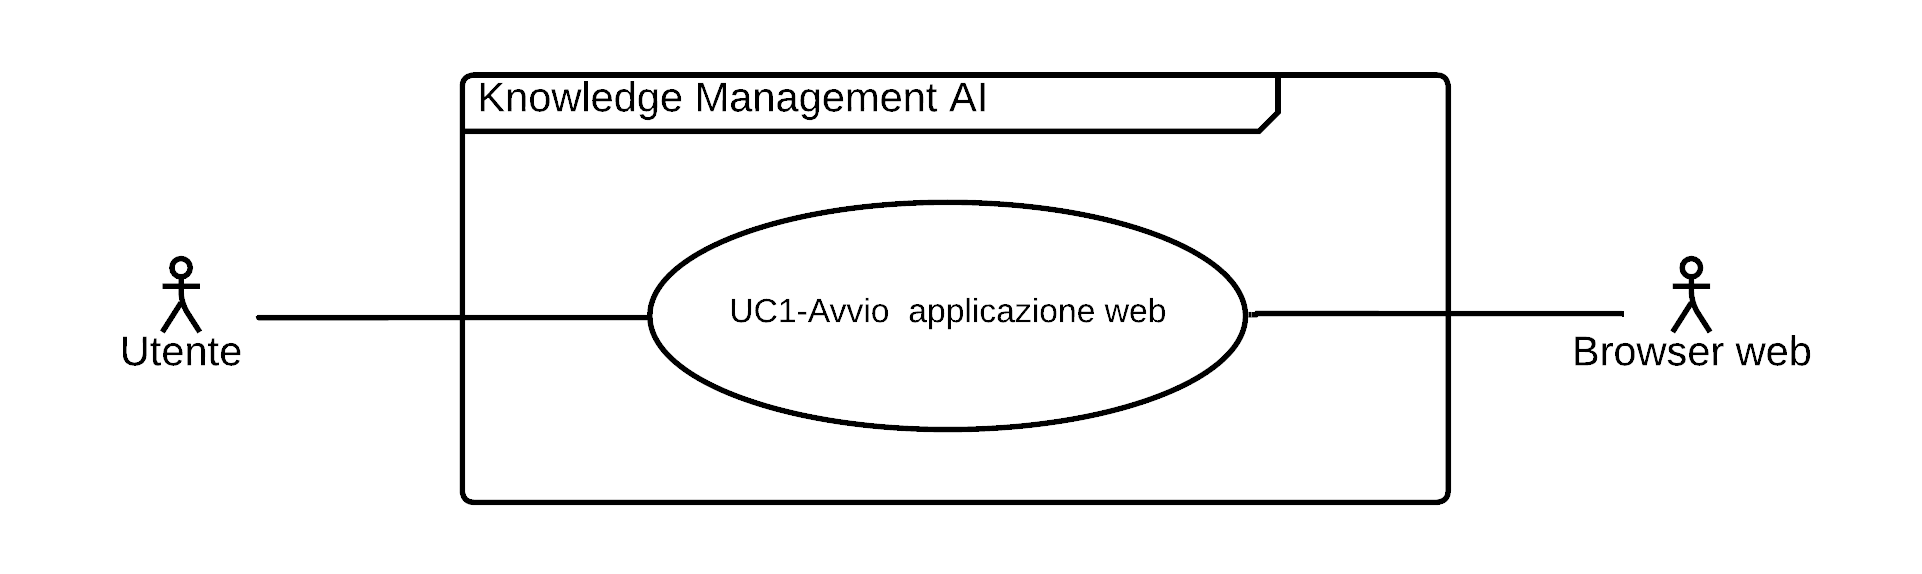
\includegraphics[width=0.75\textwidth, height=0.75\textheight, keepaspectratio]{UC-images/UC1.png}
        \caption{Diagramma del Caso d'Uso UC1}
    \end{figure}
    
    \subsubsection{UC1 - Avvio applicazione web}
    \begin{itemize}
        \item \textbf{Attore principale}: utente;
        \item \textbf{Attore secondario}: browser web;
        \item \textbf{Precondizioni}: il sistema deve essere online e l'applicazione web deve essere accessibile tramite l'URL specifico;
        \item \textbf{Postcondizioni}: l'interfaccia principale è accessibile all'utente;
        \item \textbf{Scenario principale}:
            \begin{enumerate}
                \item l'utente avvia il browser web sul proprio dispositivo;
                \item l'utente digita l'URL dell'applicazione web nella barra degli indirizzi del browser;
                \item il browser web carica la pagina iniziale dell'applicazione;
                \item l'utente visuliza l'interfaccia principale dell'applicazione.; 
            \end{enumerate}
        \item \textbf{Scenario alternativo}: se l'URL fornito dall'utente è errato o si verificano problemi di connettività, il browser web visualizza un messaggio di errore;
        \item \textbf{Trigger}: l'utente desidera avviare l'applicazione web.
    \end{itemize}

    \begin{figure}[h]
        \centering
        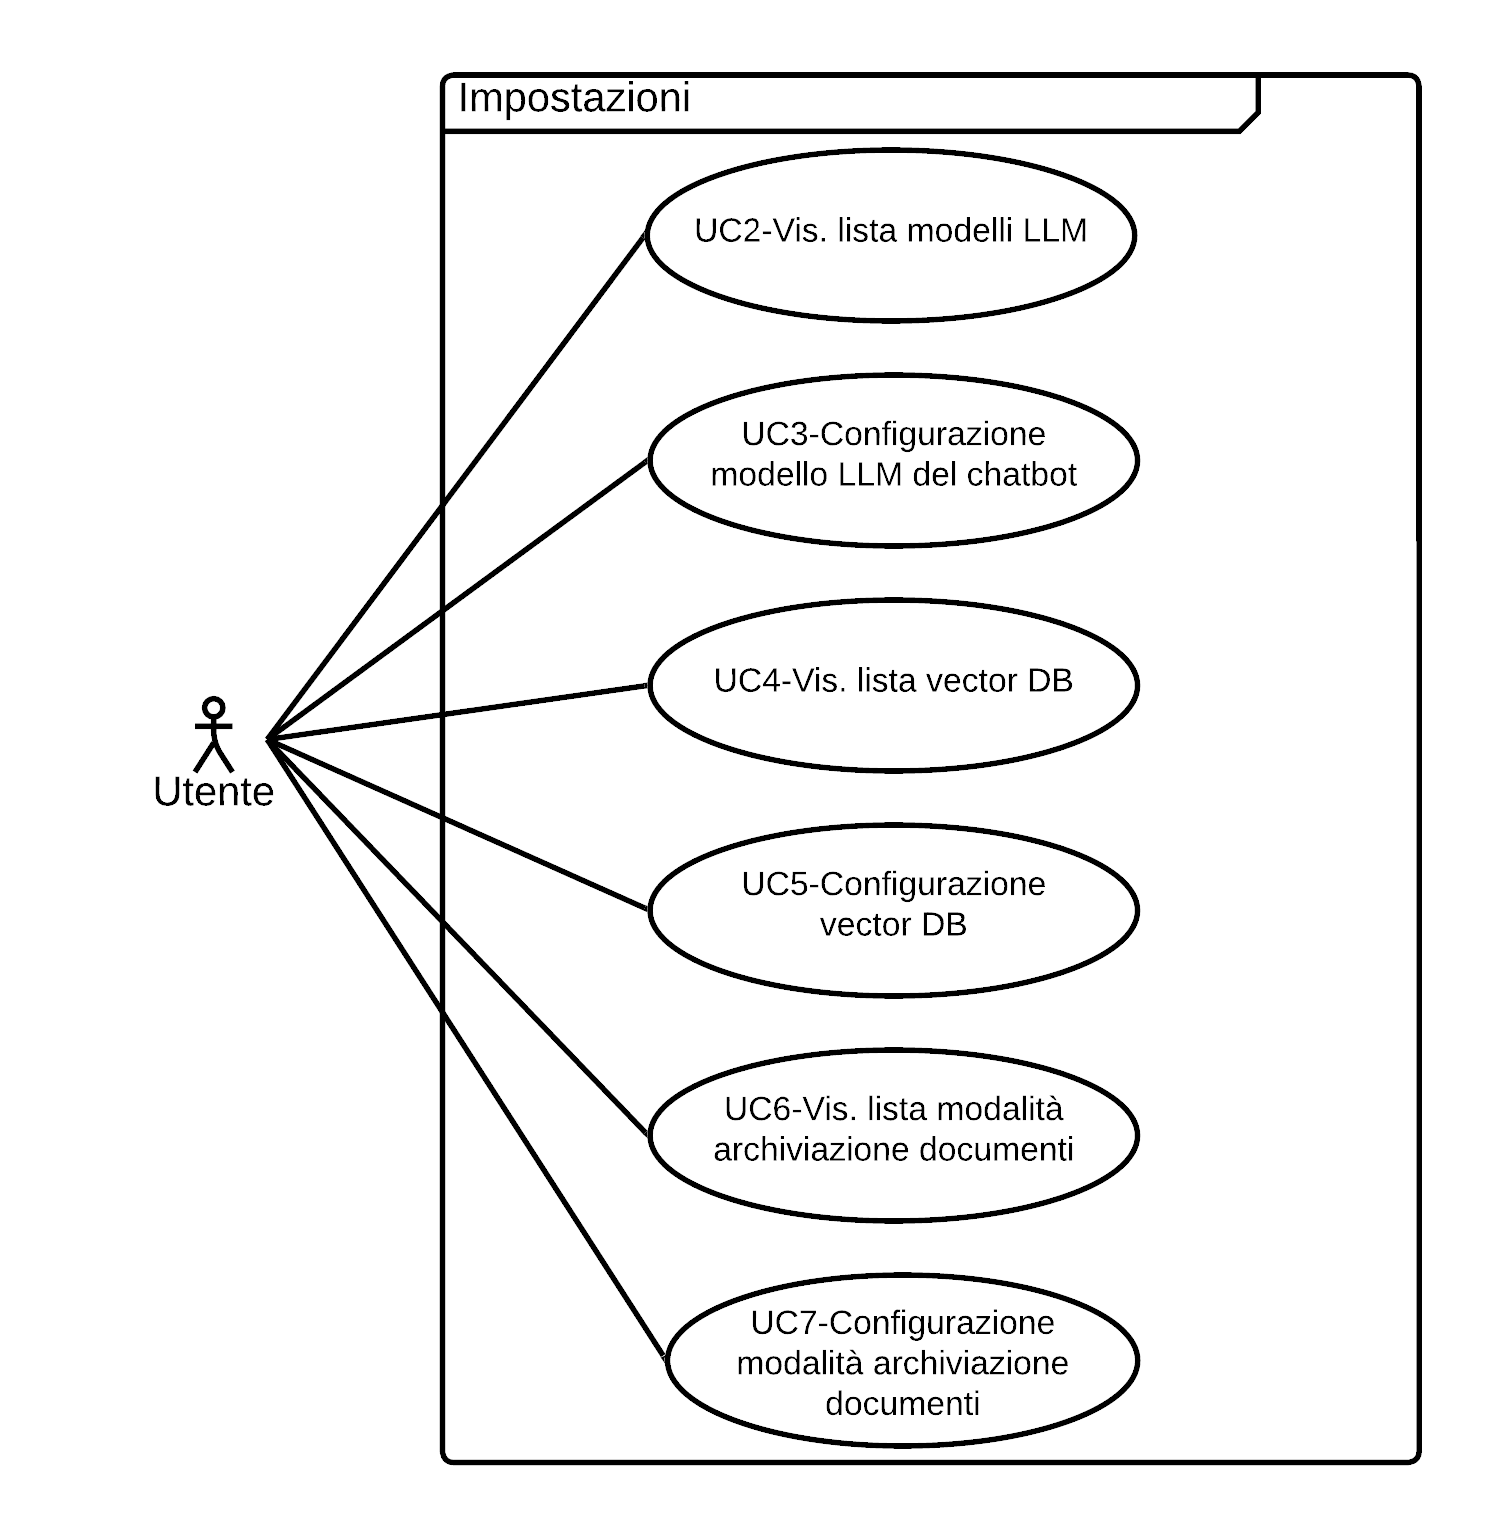
\includegraphics[width=\textwidth, height=\textheight, keepaspectratio]{UC-images/UC2-UC3-UC4-UC5-UC6-UC7.png}
        \caption{Diagramma dei Caso d'Uso UC2, UC3, UC4, UC5, UC6 e UC7}
    \end{figure}

    \subsubsection{UC2 - Visulizzazione lista modelli LLM}
    \begin{itemize}
        \item \textbf{Attore principale}: utente;
        \item \textbf{Precondizioni}: l'applicazine web è operativa e funzionante;
        \item \textbf{Postcondizioni}: 
        \begin{itemize}
            \item l'interfaccia utente è stata aggiornata per riflettere la lista dei modelli LLM;
            \item l'utente è in grado di interagire con i modelli LLM visualizzati;
            \item l'utente è a conoscenza dei modelli LLM resi disponiili dall'applicazione web.;
        \end{itemize}
        \item \textbf{Scenario principale}:
            \begin{enumerate}
                \item l'utente avvia l'applicazione web;
                \item l'utente seleziona le impostazioni dell'applicazione web;
                \item l'utente seleziona l'elenco di modelli LLM presenti nell'applicazione web.;
            \end{enumerate}
        \item \textbf{Trigger}: l'utente desidera visualizzare i modelli LLM resi disponibili dall'applicazione web.
    \end{itemize}
    
    \begin{figure}[h]
        \centering
        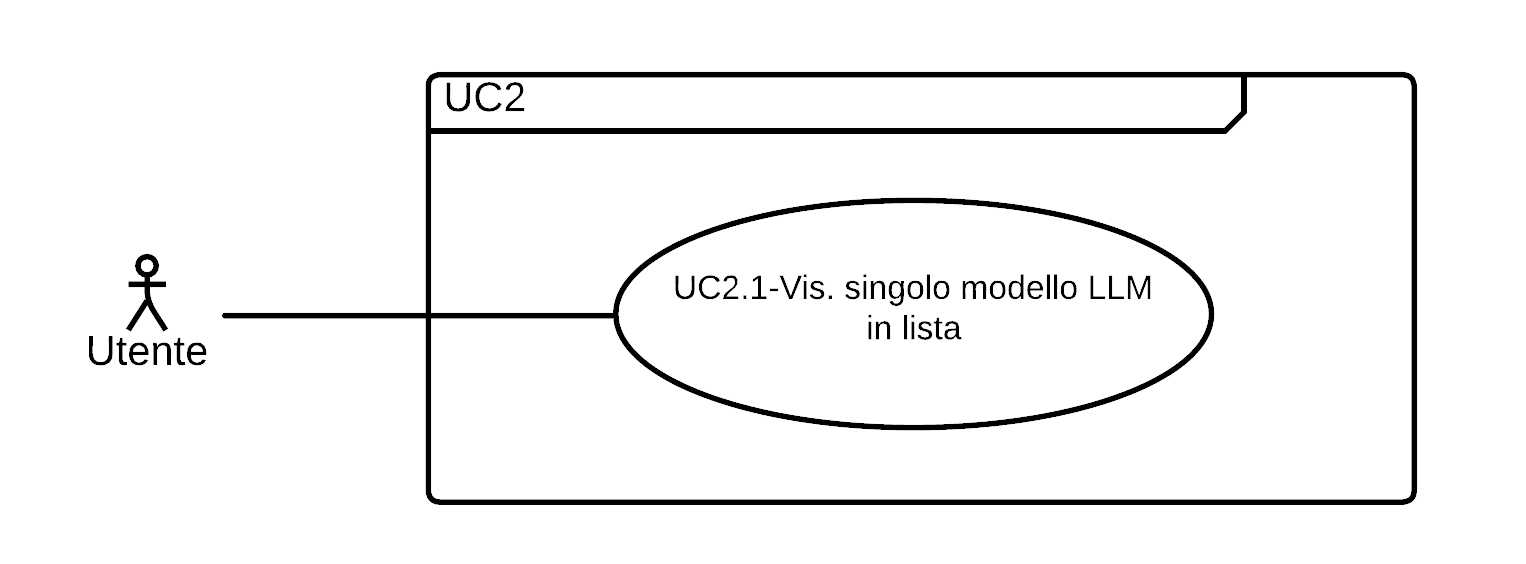
\includegraphics[width=0.5\textwidth, height=0.5\textheight, keepaspectratio]{UC-images/UC2.1.png}
        \caption{Diagramma del sotto-Caso d'Uso UC2.1}
    \end{figure}

    \subsubsection{UC2.1 - Visulizzazione singolo modelli LLM in lista}
    \begin{itemize}
        \item \textbf{Attore principale}: utente;
        \item \textbf{Precondizioni}: l'applicazine web è operativa e funzionante;
        \item \textbf{Postcondizioni}: 
        \begin{itemize}
            \item l'interfaccia utente è stata aggiornata per riflettere la lista dei modelli LLM;
            \item l'utente è in grado di interagire con i modelli LLM visualizzati;
            \item l'utente è a conoscenza di uno dei modelli LLM resi a disposizione dall'applicazione web.;
        \end{itemize} 
        \item \textbf{Scenario principale}:
            \begin{enumerate}
                \item l'utente avvia l'applicazione web;
                \item l'utente seleziona le impostazioni dell'applicazione web;
                \item l'utente seleziona l'elenco di modelli LLM presenti nell'applicazione web.;
            \end{enumerate}
        \item \textbf{Trigger}: l'utente desidera visualizzare un modello LLM tra quelli resi disponibili nella lista dall'applicazione web.
    \end{itemize}

    \begin{figure}[h]
        \centering
        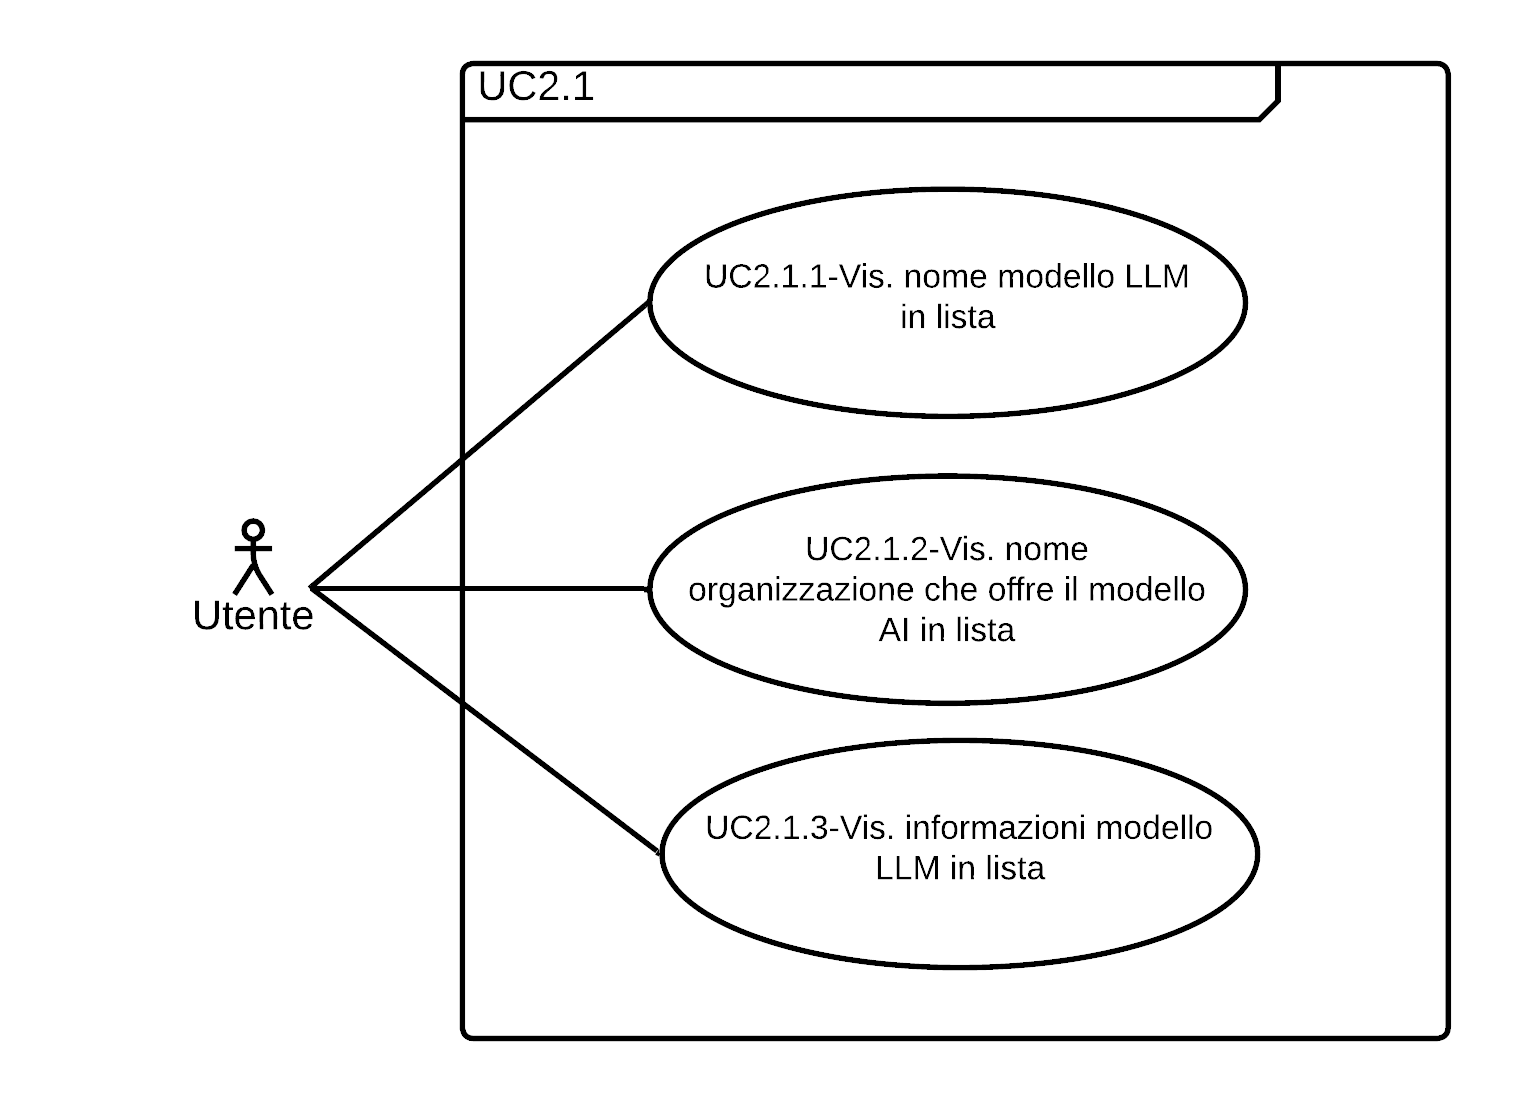
\includegraphics[width=0.75\textwidth, height=0.75\textheight, keepaspectratio]{UC-images/UC2.1.1-UC2.1.2-UC2.1.3.png}
        \caption{Diagramma dei sotto-Casi d'Uso UC2.1.1, UC2.1.2 e UC2.1.3}
    \end{figure}
        
    \subsubsection{UC2.1.1 - Visulizzazione nome modello LLM in lista}
    \begin{itemize}
        \item \textbf{Attore principale}: utente;
        \item \textbf{Precondizioni}: l'applicazine web è operativa e funzionante;
        \item \textbf{Postcondizioni}: 
        \begin{itemize}
            \item l'interfaccia utente è stata aggiornata per riflettere la lista dei modelli LLM;
            \item l'utente è in grado di interagire con i modelli LLM visualizzati;
            \item l'utente è a conoscenza del nome di uno dei modelli LLM resi a disposizione dall'applicazione web.;
        \end{itemize}  
        \item \textbf{Scenario principale}:
            \begin{enumerate}
                \item l'utente avvia l'applicazione web;
                \item l'utente seleziona le impostazioni dell'applicazione web;
                \item l'utente seleziona l'elenco di modelli LLM presenti nell'applicazione web.;
            \end{enumerate}
        \item \textbf{Trigger}: l'utente desidera visualizzare il nome di un modello LLM tra quelli resi disponibili nella lista dall'applicazione web.
    \end{itemize}

    \subsubsection{UC2.1.2 - Visulizzazione nome organizzazione che offre il modello LLM in lista}
    \begin{itemize}
        \item \textbf{Attore principale}: utente;
        \item \textbf{Precondizioni}: l'applicazine web è operativa e funzionante;
        \item \textbf{Postcondizioni}: 
        \begin{itemize}
            \item l'interfaccia utente è stata aggiornata per riflettere la lista dei modelli LLM;
            \item l'utente è in grado di interagire con i modelli LLM visualizzati;
            \item l'utente è a conoscenza del nome dell'organizzazione di uno dei modelli LLM resi a disposizione dall'applicazione web.;
        \end{itemize}
        \item \textbf{Scenario principale}:
            \begin{enumerate}
                \item l'utente avvia l'applicazione web;
                \item l'utente seleziona le impostazioni dell'applicazione web;
                \item l'utente seleziona l'elenco di modelli LLM presenti nell'applicazione web.;
            \end{enumerate}
        \item \textbf{Trigger}: l'utente desidera visualizzare il nome dell'organizzazione che offre un modello LLM tra quelli resi disponibili nella lista dall'applicazione web.
    \end{itemize}

    \subsubsection{UC2.1.3 - Visualizzazione informazioni modello LLM in lista}
    \begin{itemize}
        \item \textbf{Attore principale}: utente;
        \item \textbf{Precondizioni}: l'applicazine web è operativa e funzionante;
        \item \textbf{Postcondizioni}: 
        \begin{itemize}
            \item l'interfaccia utente è stata aggiornata per riflettere le informazioni dei modelli LLM presenti nell'applicazione web;
            \item l'utente è in grado di interagire con i modelli LLM visualizzati;
            \item l'utente è a conoscenza delle informazioni riguardanti i modelli LLM.; 
        \end{itemize}
        \item \textbf{Scenario principale}:
            \begin{enumerate}
                \item l'utente avvia l'applicazione web;
                \item l'utente seleziona le impostazioni dell'applicazione web;
                \item l'utente seleziona l'elenco dei modelli LLM presenti nell'applicazione web.;
            \end{enumerate}
        \item \textbf{Trigger}: l'utente desidera ottenere informazioni in merito ad un modello LLM reso disponibile nell'applicazione web.
    \end{itemize}
    
    \subsubsection{UC3 - Configurazione modello LLM del chatbot}
    \begin{itemize}
        \item \textbf{Attore principale}: utente;
        \item \textbf{Precondizioni}: l'applicazine web è operativa e funzionante;
        \item \textbf{Postcondizioni}: il chatbot con cui avverranno le chat aperte dall'utente si basa sul modello LLM selezionato;
        \item \textbf{Scenario principale}:
            \begin{enumerate}
                \item l'utente avvia l'applicazione web;
                \item l'utente seleziona le impostazioni dell'applicazione web;
                \item l'utente seleziona l'elenco dei modelli LLM presenti nell'applicazione web;
                \item l'utente seleziona un modello LLM tra quelli presenti nella lista;
                \item l'utente configura il modello LLM utilizzato dal chatbot.;
            \end{enumerate}
        \item \textbf{Trigger}: l'utente desidera configurare un modello LLM utilizzato dal chatbot presente nell'applicazione web.
    \end{itemize}

    \subsubsection{UC4 - Visualizzazione lista vector DB}
    \begin{itemize}
        \item \textbf{Attore principale}: utente;
        \item \textbf{Precondizioni}: l'applicazine web è operativa e funzionante;
        \item \textbf{Postcondizioni}: 
        \begin{itemize}
            \item l'interfaccia utente è stata aggiornata per riflettere la lista dei vector DB;
            \item l'utente è in grado di interagire con i vector DB visualizzati;
            \item l'utente è a conoscenza dei vector DB resi disponiili dall'applicazione web.;
        \end{itemize}
        \item \textbf{Scenario principale}:
            \begin{enumerate}
                \item l'utente avvia l'applicazione web;
                \item l'utente seleziona le impostazioni dell'applicazione web;
                \item l'utente seleziona l'elenco dei vector DB presenti nell'applicazione web.;
            \end{enumerate}
        \item \textbf{Trigger}: l'utente desidera visualizzare i vector DB resi disponibili dall'applicazione web.
    \end{itemize}

    \begin{figure}[h]
        \centering
        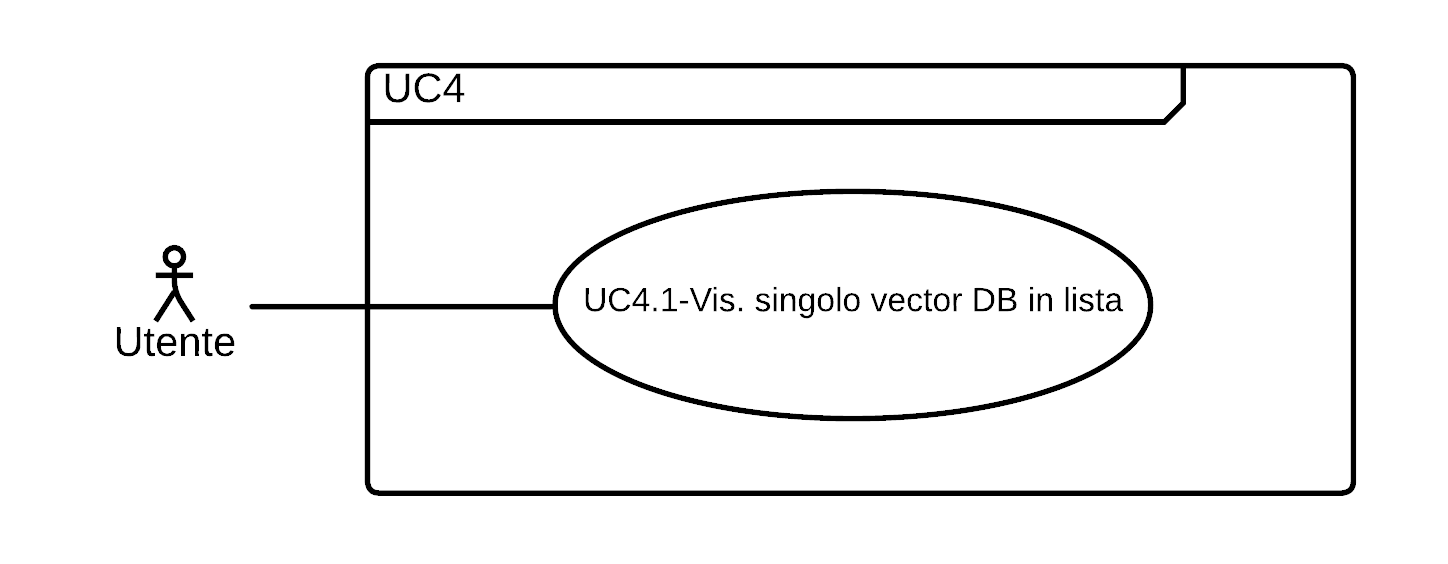
\includegraphics[width=0.5\textwidth, height=0.5\textheight, keepaspectratio]{UC-images/UC4.1.png}
        \caption{Diagramma del sotto-Caso d'Uso UC4.1}
    \end{figure}

    \subsubsection{UC4.1 - Visulizzazione singolo vector DB in lista}
    \begin{itemize}
        \item \textbf{Attore principale}: utente;
        \item \textbf{Precondizioni}: l'applicazine web è operativa e funzionante;
        \item \textbf{Postcondizioni}: 
        \begin{itemize}
            \item l'interfaccia utente è stata aggiornata per riflettere la lista dei vector DB;
            \item l'utente è in grado di interagire con i vector DB visualizzati;
            \item l'utente è a conoscenza di uno dei vector DB resi a disposizione dall'applicazione web.;
        \end{itemize} 
        \item \textbf{Scenario principale}:
            \begin{enumerate}
                \item l'utente avvia l'applicazione web;
                \item l'utente seleziona le impostazioni dell'applicazione web;
                \item l'utente seleziona l'elenco di vector DB presenti nell'applicazione web.;
            \end{enumerate}
        \item \textbf{Trigger}: l'utente desidera visualizzare un vector DB tra quelli resi disponibili nella lista dall'applicazione web.
    \end{itemize}

    \begin{figure}[h]
        \centering
        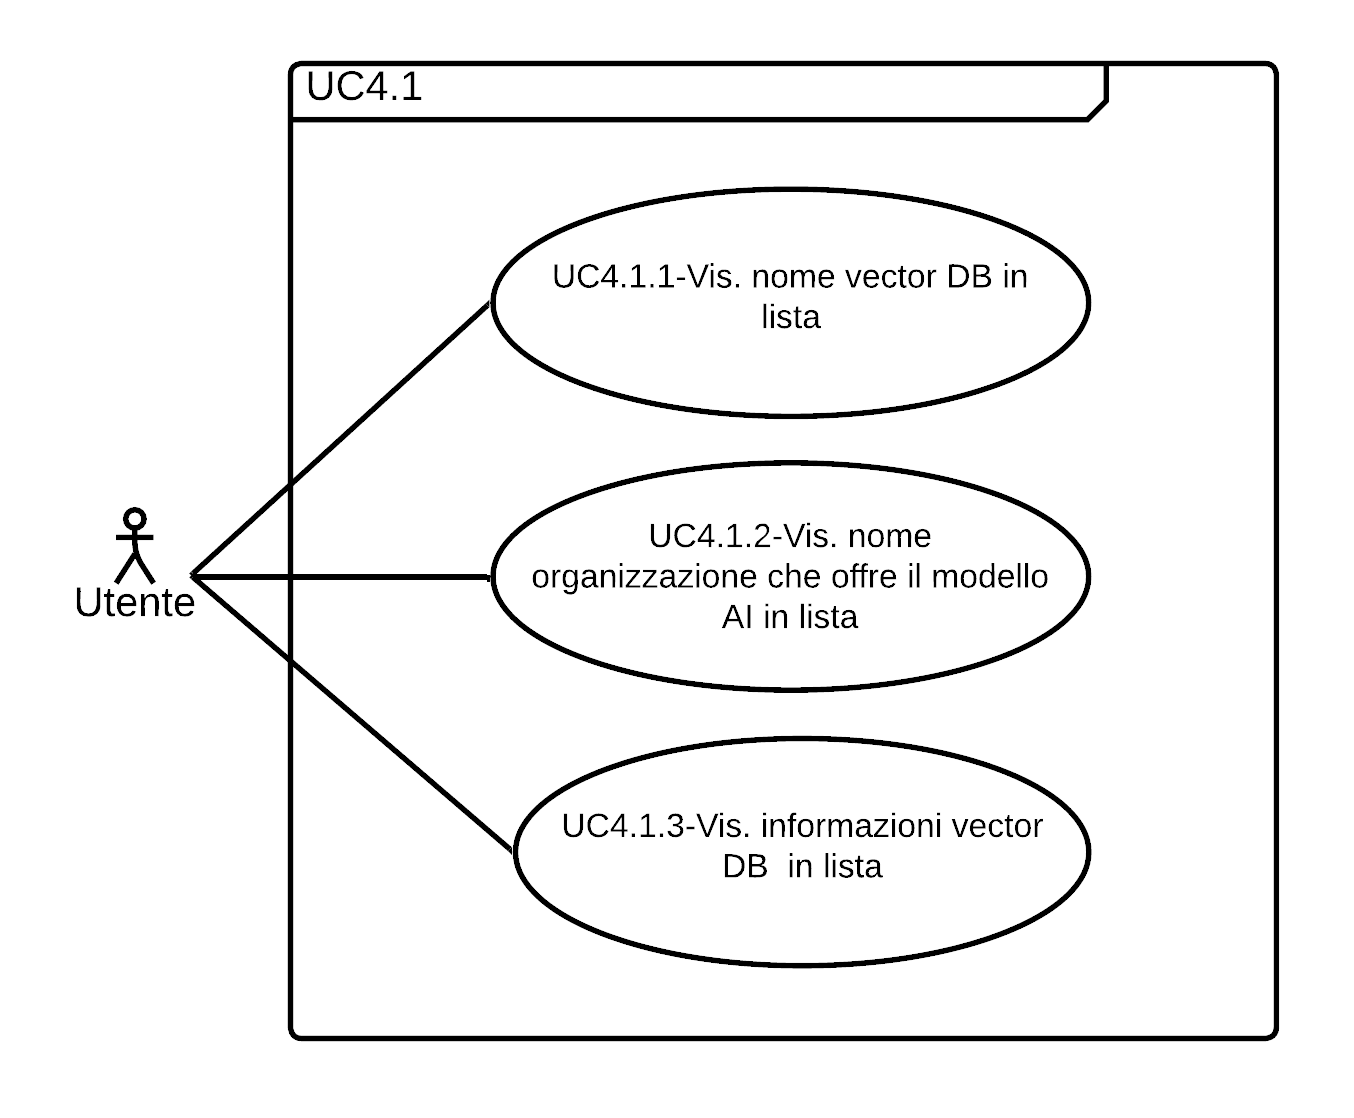
\includegraphics[width=0.75\textwidth, height=0.75\textheight, keepaspectratio]{UC-images/UC4.1.1-UC4.1.2-UC4.1.3.png}
        \caption{Diagramma dei sotto-Casi d'Uso UC4.1.1, UC4.1.2 e UC4.1.3}
    \end{figure}
        
    \subsubsection{UC4.1.1 - Visulizzazione nome vector DB in lista}
    \begin{itemize}
        \item \textbf{Attore principale}: utente;
        \item \textbf{Precondizioni}: l'applicazine web è operativa e funzionante;
        \item \textbf{Postcondizioni}: 
        \begin{itemize}
            \item l'interfaccia utente è stata aggiornata per riflettere la lista dei vector DB;
            \item l'utente è in grado di interagire con i vector DB visualizzati;
            \item l'utente è a conoscenza del nome di uno dei vector DB resi a disposizione dall'applicazione web.;
        \end{itemize}  
        \item \textbf{Scenario principale}:
            \begin{enumerate}
                \item l'utente avvia l'applicazione web;
                \item l'utente seleziona le impostazioni dell'applicazione web;
                \item l'utente seleziona l'elenco di vector DB presenti nell'applicazione web.;
            \end{enumerate}
        \item \textbf{Trigger}: l'utente desidera visualizzare il nome di un vector DB tra quelli resi disponibili nella lista dall'applicazione web.
    \end{itemize}

    \subsubsection{UC4.1.2 - Visulizzazione nome organizzazione che offre il vector DB in lista}
    \begin{itemize}
        \item \textbf{Attore principale}: utente;
        \item \textbf{Precondizioni}: l'applicazine web è operativa e funzionante;
        \item \textbf{Postcondizioni}: 
        \begin{itemize}
            \item l'interfaccia utente è stata aggiornata per riflettere la lista dei vector DB;
            \item l'utente è in grado di interagire con i vector DB visualizzati;
            \item l'utente è a conoscenza del nome dell'organizzazione di uno dei vector DB resi a disposizione dall'applicazione web.;
        \end{itemize}
        \item \textbf{Scenario principale}:
            \begin{enumerate}
                \item l'utente avvia l'applicazione web;
                \item l'utente seleziona le impostazioni dell'applicazione web;
                \item l'utente seleziona l'elenco di vector DB presenti nell'applicazione web.;
            \end{enumerate}
        \item \textbf{Trigger}: l'utente desidera visualizzare il nome dell'organizzazione che offre un vector DB tra quelli resi disponibili nella lista dall'applicazione web.
    \end{itemize}

    \subsubsection{UC4.1.3 - Visualizzazione informazioni vector DB in lista}
    \begin{itemize}
        \item \textbf{Attore principale}: utente;
        \item \textbf{Precondizioni}: l'applicazine web è operativa e funzionante;
        \item \textbf{Postcondizioni}: 
        \begin{itemize}
            \item l'interfaccia utente è stata aggiornata per riflettere le informazioni dei vector DB presenti nell'applicazione web;
            \item l'utente è a conoscenza delle informazioni riguardanti i vector DB.; 
        \end{itemize}
        \item \textbf{Scenario principale}:
            \begin{enumerate}
                \item l'utente avvia l'applicazione web;
                \item l'utente seleziona le impostazioni dell'applicazione web;
                \item l'utente seleziona l'elenco dei vector DB presenti nell'applicazione web.;
            \end{enumerate}
        \item \textbf{Trigger}: l'utente desidera ottenere informazioni in merito ad un vector DB reso disponibile nell'applicazione web.
    \end{itemize}

    \subsubsection{UC5 - Configurazione vector DB}
    \begin{itemize}
        \item \textbf{Attore principale}: utente;
        \item \textbf{Precondizioni}: l'applicazine web è operativa e funzionante;
        \item \textbf{Postcondizioni}: l'applicazione web utilizza il vector DB selezionato dall'utente;
        \item \textbf{Scenario principale}:
            \begin{enumerate}
                \item l'utente avvia l'applicazione web;
                \item l'utente seleziona le impostazioni dell'applicazione web;
                \item l'utente seleziona l'elenco dei vector DB presenti nell'applicazione web;
                \item l'utente seleziona un vector DB tra quelli presenti nella lista;
                \item l'utente configura il vector DB utilizzato dall'applicazione web.;
            \end{enumerate}
        \item \textbf{Trigger}: l'utente desidera configurare il vector DB utilizzato dall'applicazione web.
    \end{itemize}

    \subsubsection{UC6 - Visualizzazione lista modalità archiviazione documenti}
    \begin{itemize}
        \item \textbf{Attore principale}: utente;
        \item \textbf{Precondizioni}: l'applicazine web è operativa e funzionante;
        \item \textbf{Postcondizioni}: 
        \begin{itemize}
            \item l'interfaccia utente è stata aggiornata per riflettere la lista delle modalità di archiviazione dei documenti;
            \item l'utente è in grado di interagire con le modalità di archiviazione dei documenti visualizzati;
            \item l'utente è a conoscenza delle modalità di archiviazione dei documenti resi disponiili dall'applicazione web.;
        \end{itemize}
        \item \textbf{Scenario principale}:
            \begin{enumerate}
                \item l'utente avvia l'applicazione web;
                \item l'utente seleziona le impostazioni dell'applicazione web;
                \item l'utente seleziona l'elenco delle modalità di archiviazione dei documenti presenti nell'applicazione web.;
            \end{enumerate}
        \item \textbf{Trigger}: l'utente desidera visualizzare le modalità di archiviazione dei documenti resi disponibili dall'applicazione web.
    \end{itemize}

    \begin{figure}[h]
        \centering
        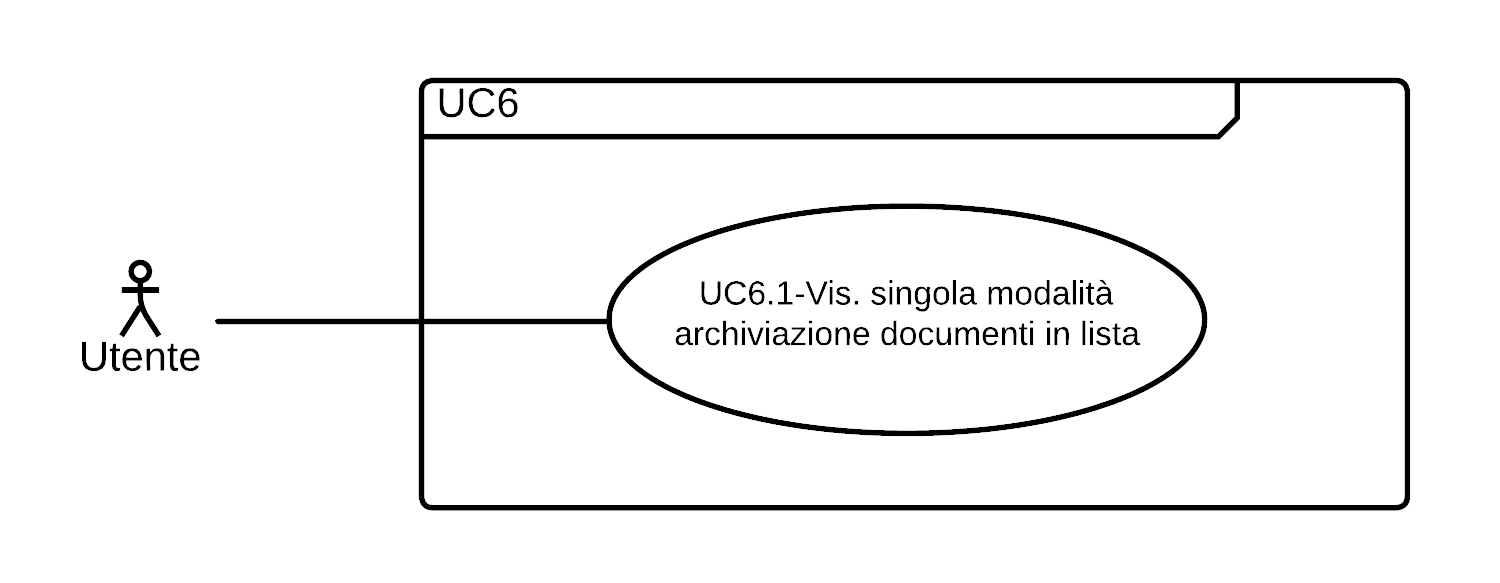
\includegraphics[width=0.5\textwidth, height=0.5\textheight, keepaspectratio]{UC-images/UC6.1.png}
        \caption{Diagramma del sotto-Caso d'Uso UC6.1}
    \end{figure}

    \subsubsection{UC6.1 - Visulizzazione singola modalità archiviazione documenti in lista}
    \begin{itemize}
        \item \textbf{Attore principale}: utente;
        \item \textbf{Precondizioni}: l'applicazine web è operativa e funzionante;
        \item \textbf{Postcondizioni}: 
        \begin{itemize}
            \item l'interfaccia utente è stata aggiornata per riflettere la lista delle modalità di archiviazione dei documenti;
            \item l'utente è in grado di interagire con le modalità di archiviazione dei documenti visualizzati;
            \item l'utente è a conoscenza di una deile modalità di archiviazione dei documenti resi a disposizione dall'applicazione web.;
        \end{itemize} 
        \item \textbf{Scenario principale}:
            \begin{enumerate}
                \item l'utente avvia l'applicazione web;
                \item l'utente seleziona le impostazioni dell'applicazione web;
                \item l'utente seleziona l'elenco delle modalità di archiviazione dei documenti presente nell'applicazione web.;
            \end{enumerate}
        \item \textbf{Trigger}: l'utente desidera visualizzare una modalità di archiviazione dei documenti tra quelle rese disponibili nella lista dall'applicazione web.
    \end{itemize}

    \begin{figure}[h]
        \centering
        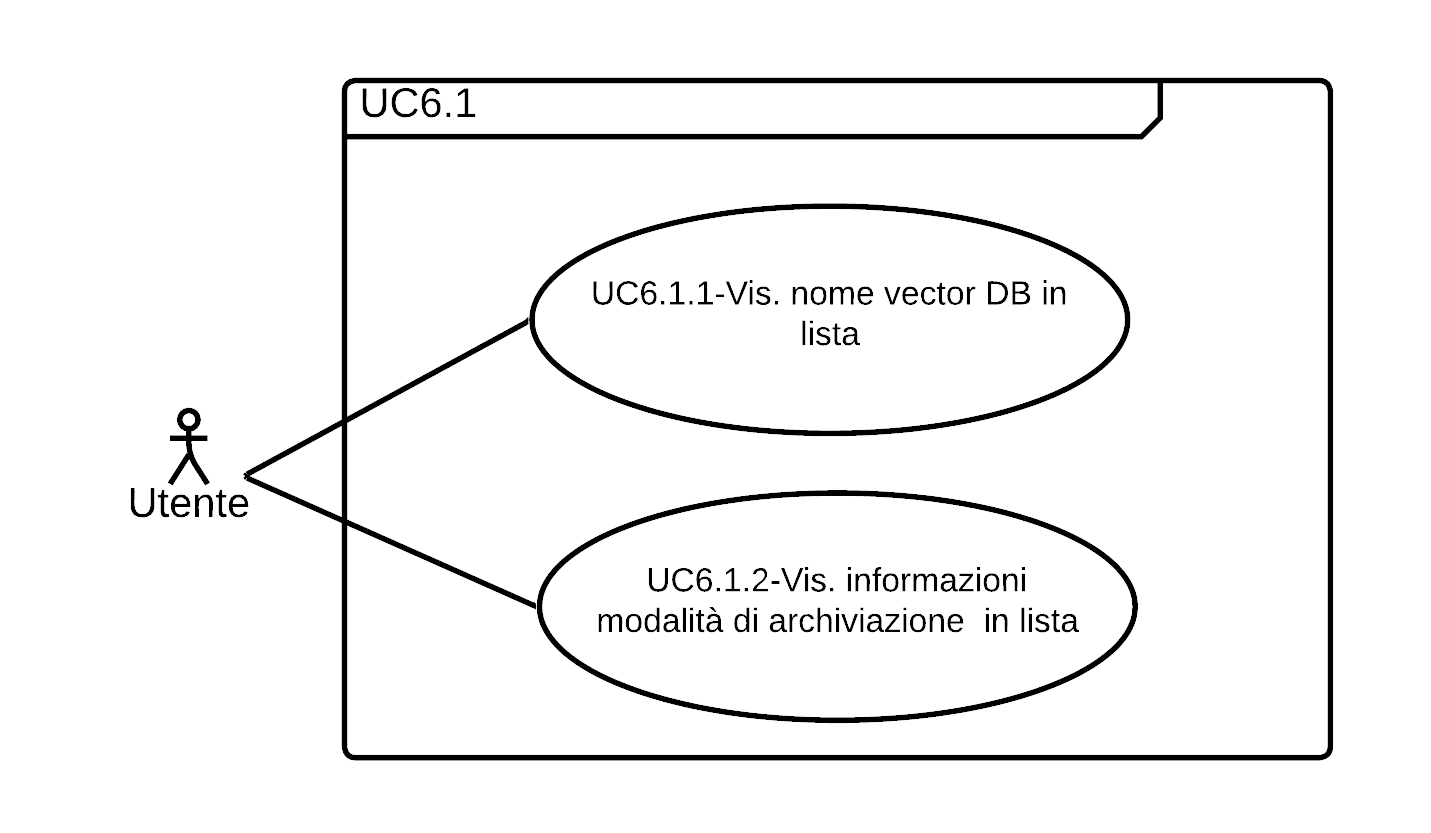
\includegraphics[width=0.75\textwidth, height=0.75\textheight, keepaspectratio]{UC-images/UC6.1.1-UC6.1.2.png}
        \caption{Diagramma dei sotto-Casi d'Uso UC6.1.1 e UC6.1.2}
    \end{figure}
        
    \subsubsection{UC6.1.1 - Visulizzazione nome modalità archiviazione documenti in lista}
    \begin{itemize}
        \item \textbf{Attore principale}: utente;
        \item \textbf{Precondizioni}: l'applicazine web è operativa e funzionante;
        \item \textbf{Postcondizioni}: 
        \begin{itemize}
            \item l'interfaccia utente è stata aggiornata per riflettere la lista delle modalità di archiviazione dei documenti;
            \item l'utente è in grado di interagire con le modalità di archiviazione dei documenti visualizzati;
            \item l'utente è a conoscenza del nome di una delle modalità di archiviazione dei documenti resi a disposizione dall'applicazione web.;
        \end{itemize}  
        \item \textbf{Scenario principale}:
            \begin{enumerate}
                \item l'utente avvia l'applicazione web;
                \item l'utente seleziona le impostazioni dell'applicazione web;
                \item l'utente seleziona l'elenco delle modalità di archiviazione dei documenti presente nell'applicazione web.;
            \end{enumerate}
        \item \textbf{Trigger}: l'utente desidera visualizzare il nome di una modalità di archiviazione dei documenti tra quelle rese disponibili nella lista dall'applicazione web.
    \end{itemize}

    \subsubsection{UC6.1.2 - Visualizzazione informazioni modalità archiviazione documenti in lista}
    \begin{itemize}
        \item \textbf{Attore principale}: utente;
        \item \textbf{Precondizioni}: l'applicazine web è operativa e funzionante;
        \item \textbf{Postcondizioni}: 
        \begin{itemize}
            \item l'interfaccia utente è stata aggiornata per riflettere le informazioni delle modalità di archiviazione dei documenti presenti nell'applicazione web;
            \item l'utente è a conoscenza delle informazioni riguardanti le modalità di archiviazione dei documenti.; 
        \end{itemize}
        \item \textbf{Scenario principale}:
            \begin{enumerate}
                \item l'utente avvia l'applicazione web;
                \item l'utente seleziona le impostazioni dell'applicazione web;
                \item l'utente seleziona l'elenco delle modalità di archiviazione dei documenti presente nell'applicazione web.;
            \end{enumerate}
        \item \textbf{Trigger}: l'utente desidera ottenere informazioni in merito ad una modalità di archiviazione dei documenti resa disponibile nell'applicazione web.
    \end{itemize}

    \subsubsection{UC7 - Configurazione modalità archiviazione documenti}
    \begin{itemize}
        \item \textbf{Attore principale}: utente;
        \item \textbf{Precondizioni}: l'applicazine web è operativa e funzionante;
        \item \textbf{Postcondizioni}: l'applicazione web utilizza la modalità di archiviazione dei documenti selezionata dall'utente;
        \item \textbf{Scenario principale}:
            \begin{enumerate}
                \item l'utente avvia l'applicazione web;
                \item l'utente seleziona le impostazioni dell'applicazione web;
                \item l'utente seleziona l'elenco delle modalità di archiviazione dei documenti presente nell'applicazione web;
                \item l'utente seleziona una modalità di archiviazione dei documenti tra quelle presenti nella lista;
                \item l'utente configura la modalità di archiviazione dei documenti utilizzata nell'applicazione web.;
            \end{enumerate}
        \item \textbf{Trigger}: l'utente desidera configurare la modalità di archiviazione dei documenti utilizzata dall'applicazione web.
    \end{itemize}

    \begin{figure}[h]
        \centering
        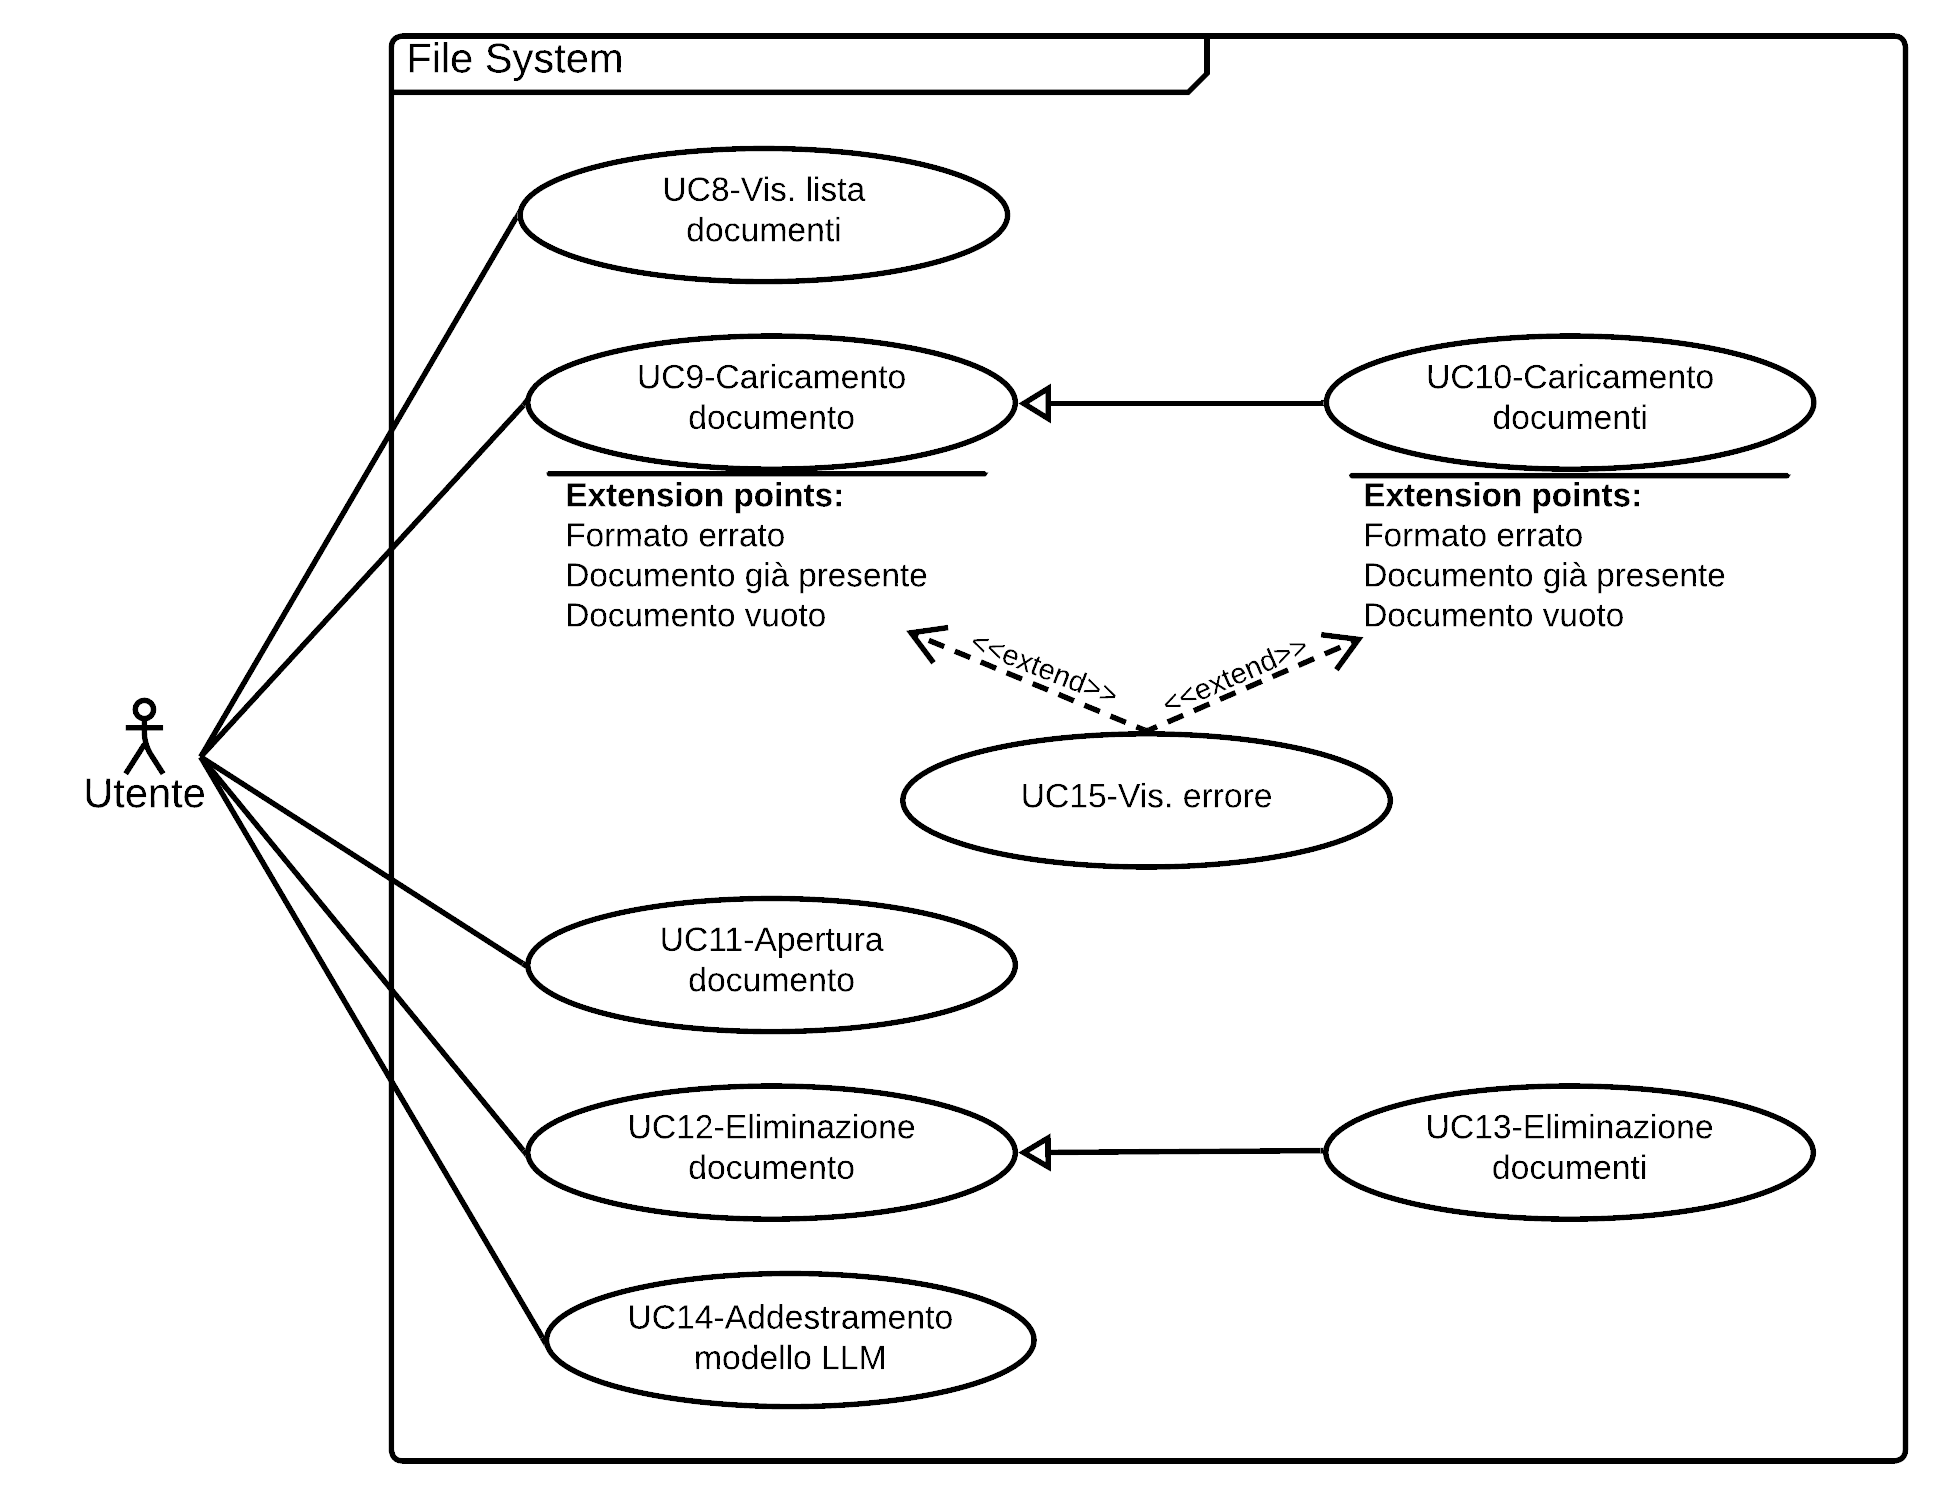
\includegraphics[width=\textwidth, height=\textheight, keepaspectratio]{UC-images/UC8-UC9-UC10-UC11-UC12-UC13-UC14-UC15.png}
        \caption{Diagramma dei Caso d'Uso UC8, UC9, UC10, UC11, UC12, UC13, UC14 e UC15}
    \end{figure}

    \subsubsection{UC8 - Visualizzazione lista documenti}
    \begin{itemize}
        \item \textbf{Attore principale}: utente;
        \item \textbf{Precondizioni}: l'applicazine web è operativa e funzionante;
        \item \textbf{Postcondizioni}:
        \begin{itemize}
            \item l'interfaccia utente è stata aggiornata per riflettere la lista dei documenti presenti nell'applicazione web;
            \item l'utente è a conoscenza dei file presenti nell'applicazione web.;
        \end{itemize} 
        \item \textbf{Scenario principale}:
        \begin{enumerate}
            \item l'utente avvia l'applicazione web;
            \item l'utente visualizza la lista dei documenti presenti nell'applicazione web.;
        \end{enumerate}
        \item \textbf{Trigger}: l'utente desidera visualizzare i documenti caricati nell'applicazione web.
    \end{itemize}

    \begin{figure}[h]
        \centering
        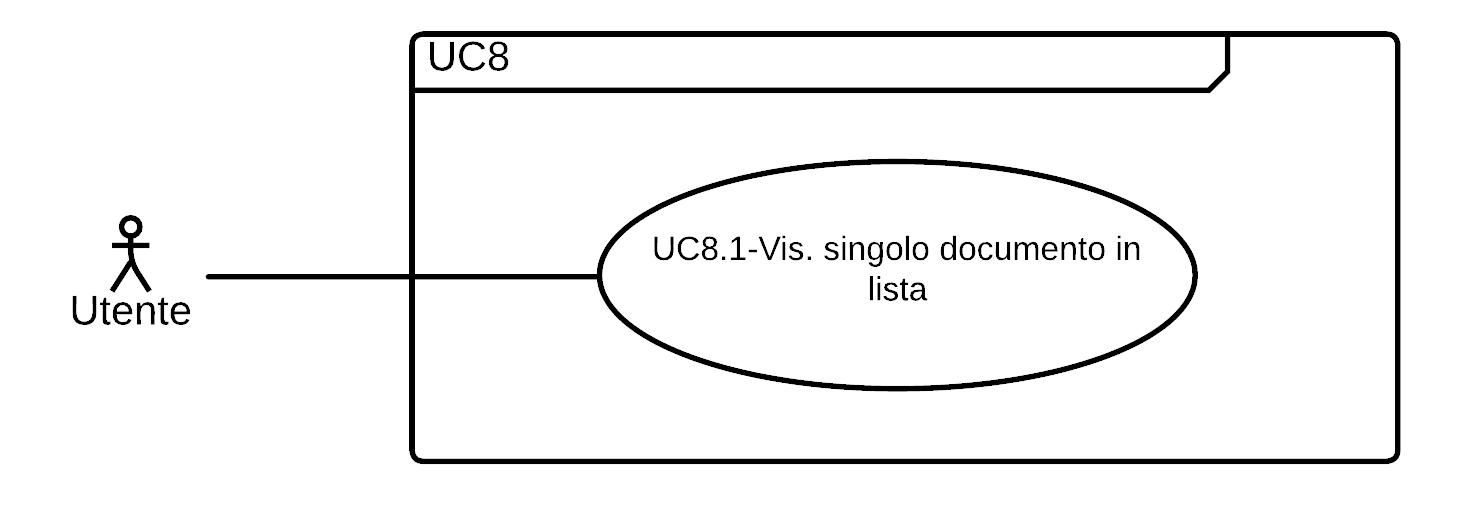
\includegraphics[width=0.75\textwidth, height=0.75\textheight, keepaspectratio]{UC-images/UC8.1.png}
        \caption{Diagramma del sotto-Caso d'Uso UC8.1}
    \end{figure}
    
    \subsubsection{UC8.1 - Visualizzazione singolo documento in lista}
    \begin{itemize}
        \item \textbf{Attore principale}: utente;
        \item \textbf{Precondizioni}: l'applicazine web è operativa e funzionante;
        \item \textbf{Postcondizioni}:
        \begin{itemize}
            \item l'interfaccia utente è stata aggiornata per riflettere la lista dei documenti presenti nell'applicazione web;
            \item l'utente è a conoscenza di un file presente nell'applicazione web.;
        \end{itemize}
        \item \textbf{Scenario principale}:
        \begin{enumerate}
            \item l'utente avvia l'applicazione web;
            \item l'utente visualizza la lista dei documenti presenti nell'applicazione web.;
        \end{enumerate}
        \item \textbf{Trigger}: l'utente desidera visualizzare un singolo documento caricato nell'applicazione web.
    \end{itemize}

    \begin{figure}[h]
        \centering
        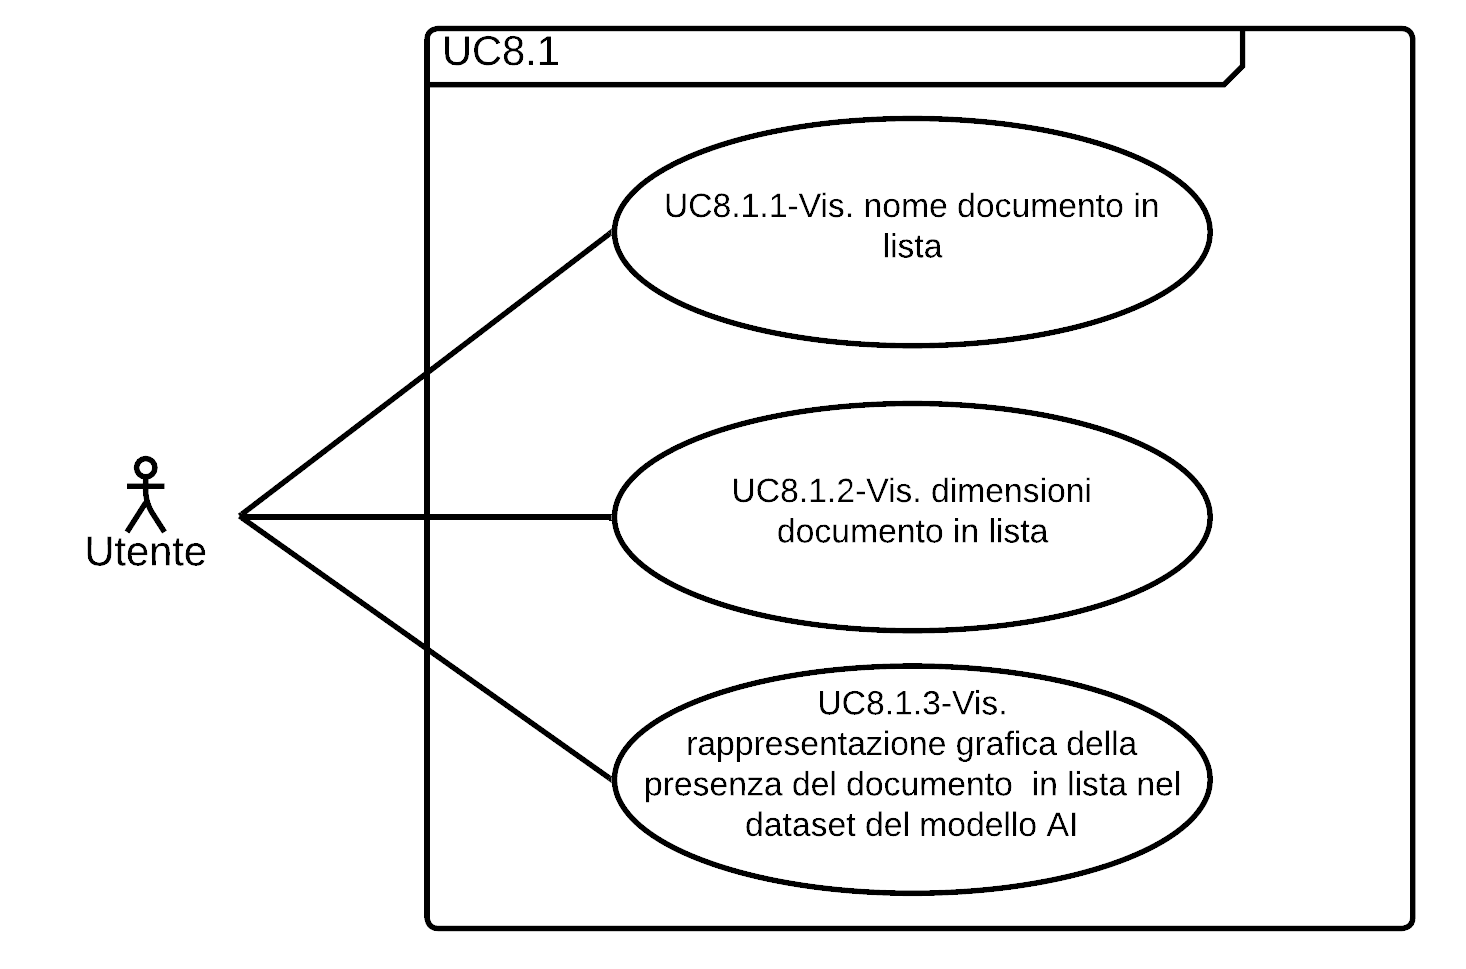
\includegraphics[width=0.75\textwidth, height=0.75\textheight, keepaspectratio]{UC-images/UC8.1.1-UC8.1.2-UC8.1.3.png}
        \caption{Diagramma dei sotto-Casi d'Uso UC8.1.1, UC8.1.2 e UC8.1.3}
    \end{figure}
    
    \subsubsection{UC8.1.1 - Visualizzazione nome documento in lista}
    \begin{itemize}
        \item \textbf{Attore principale}: utente;
        \item \textbf{Precondizioni}: l'applicazine web è operativa e funzionante;
        \item \textbf{Postcondizioni}:
        \begin{itemize}
            \item l'interfaccia utente è stata aggiornata per riflettere la lista dei documenti presenti nell'applicazione web;
            \item l'utente è a conoscenza del nome di un file presente nell'applicazione web.;
        \end{itemize}
        \item \textbf{Scenario principale}:
        \begin{enumerate}
            \item l'utente avvia l'applicazione web;
            \item l'utente visualizza la lista dei documenti presenti nell'applicazione web.;
        \end{enumerate}
        \item \textbf{Trigger}: l'utente desidera visualizzare il nome di un singolo documento caricato nell'applicazione web.
    \end{itemize}

    \subsubsection{UC8.1.2 - Visualizzazione dimensioni documento in lista}
    \begin{itemize}
        \item \textbf{Attore principale}: utente;
        \item \textbf{Precondizioni}: l'applicazine web è operativa e funzionante;
        \item \textbf{Postcondizioni}:
        \begin{itemize}
            \item l'interfaccia utente è stata aggiornata per riflettere la lista dei documenti presenti nell'applicazione web;
            \item l'utente è a conoscenza delle dimensioni di un file presente nell'applicazione web.;
        \end{itemize}
        \item \textbf{Scenario principale}:
        \begin{enumerate}
            \item l'utente avvia l'applicazione web;
            \item l'utente visualizza la lista dei documenti presenti nell'applicazione web.;
        \end{enumerate}
        \item \textbf{Trigger}: l'utente desidera visualizzare le dimensioni di un singolo documento caricato nell'applicazione web.
    \end{itemize}

    \subsubsection{UC8.1.3 - Visualizzazione rappresentazione grafica della presenza di un documento in lista nel dataset del modello AI}
    \begin{itemize}
        \item \textbf{Attore principale}: utente;
        \item \textbf{Precondizioni}: l'applicazine web è operativa e funzionante;
        \item \textbf{Postcondizioni}:
        \begin{itemize}
            \item l'interfaccia utente è stata aggiornata per riflettere la lista dei documenti presenti nell'applicazione web;
            \item l'utente è a conoscenza della preseza o meno di un file caricato nell'applicazione web all'interno del dataset di un modello LLM.;
        \end{itemize}
        \item \textbf{Scenario principale}:
        \begin{enumerate}
            \item l'utente avvia l'applicazione web;
            \item l'utente visualizza la lista dei documenti presenti nell'applicazione web.;
        \end{enumerate}
        \item \textbf{Trigger}: l'utente desidera visualizzare la presenza o meno di un singolo documento caricato nell'applicazione web all'interno del dataset di un modello LLM.
    \end{itemize}
        
    \subsubsection{UC9 - Caricamento documento} 
    \begin{itemize}
        \item \textbf{Attore principale}: utente;
        \item \textbf{Precondizioni}: l'applicazine web è operativa e funzionante;
        \item \textbf{Postcondizioni}: il documento desiderato dall'utente è ora presente nell'applicazione web;
        \item \textbf{Scenario principale}:
            \begin{enumerate}
                \item l'utente avvia l'applicazione web;
                \item l'utente seleziona il documento che desidera caricare tramite un'interfaccia di selezione file;
                \item il documento viene caricato nell'applicazione web.;
            \end{enumerate}
        \item \textbf{Scenario alternativo}:
            \begin{itemize}
                \item l'utente carica un file non supportato;
                \item l'utente carica un file già presente nell'applicazione web;
                \item l'utente carica un file vuoto.;
            \end{itemize}
        \item \textbf{Trigger}: l'utente desidera caricare un documento nell'applicazione web.
    \end{itemize}

    \begin{figure}[h]
        \centering
        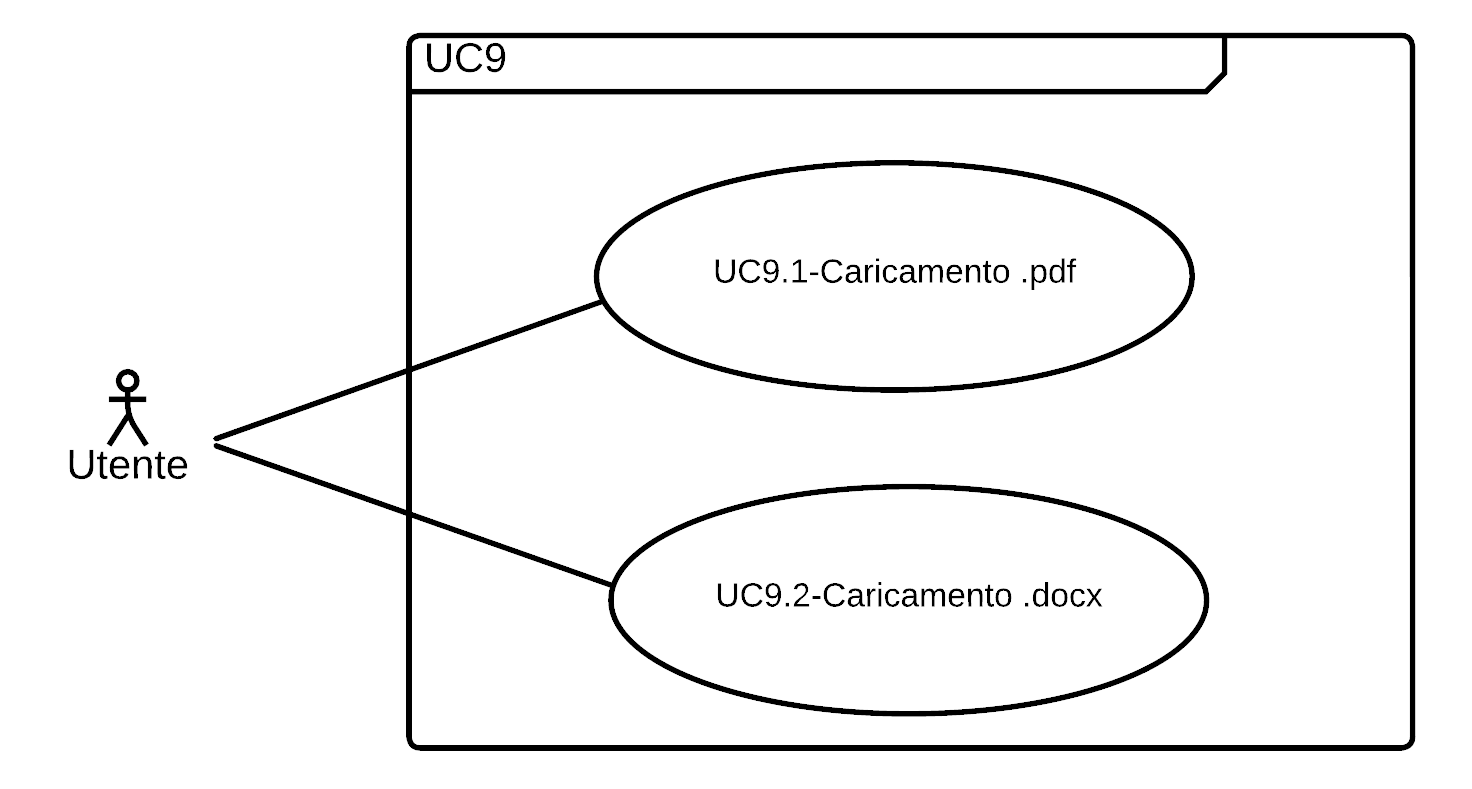
\includegraphics[width=0.6\textwidth, height=0.6\textheight, keepaspectratio]{UC-images/UC9.1-UC9.2.png}
        \caption{Diagramma dei sotto-Casi d'Uso UC9.1 e UC9.2}
    \end{figure}
    
    \subsubsection{UC9.1 - Caricamento .pdf}
    \begin{itemize}
        \item \textbf{Attore principale}: utente;
        \item \textbf{Precondizioni}: l'applicazine web è operativa e funzionante;
        \item \textbf{Postcondizioni}: il documento.pdf desiderato dall'utente è ora presente nell'applicazione web;
        \item \textbf{Scenario principale}:
            \begin{enumerate}
                \item l'utente avvia l'applicazione web;
                \item l'utente seleziona il documento.pdf che desidera caricare tramite un'interfaccia di selezione file;
                \item il documento.pdf viene caricato nell'applicazione web.;
            \end{enumerate}
        \item \textbf{Trigger}: l'utente desidera caricare un documento.pdf nell'applicazione web.
    \end{itemize}

    \subsubsection{UC9.2 - Caricamento .docx}
    \begin{itemize}
        \item \textbf{Attore principale}: utente;
        \item \textbf{Precondizioni}: l'applicazine web è operativa e funzionante;
        \item \textbf{Postcondizioni}: il documento.docx desiderato dall'utente è ora presente nell'applicazione web;
        \item \textbf{Scenario principale}:
            \begin{enumerate}
                \item l'utente avvia l'applicazione web;
                \item l'utente seleziona il documento.docx che desidera caricare tramite un'interfaccia di selezione file;
                \item il documento.docx viene caricato nell'applicazione web.;
            \end{enumerate}
        \item \textbf{Trigger}: l'utente desidera caricare un documento.docx nell'applicazione web.
    \end{itemize}

    \subsubsection{UC10 - Caricamento documenti} 
    \begin{itemize}
        \item \textbf{Attore principale}: utente;
        \item \textbf{Precondizioni}: l'applicazine web è operativa e funzionante;
        \item \textbf{Postcondizioni}: i file selezionati dall'utente sono ora caricati nell'applicazione web;
        \item \textbf{Scenario principale}:
            \begin{enumerate}
                \item l'utente avvia l'applicazione web;
                \item l'utente seleziona un documento che desidera caricare tramite un'interfaccia di selezione file;
                \item l'utente seleziona l'opzione di caricamento di ulteriori file e seleziona i restanti file che vuole caricare;
                \item i documenti vengono caricati nell'applicazione web.;
            \end{enumerate}
        \item \textbf{Scenario secondario}:
            \begin{itemize}
                \item l'utente carica uno o più file non supportato/i;
                \item l'utente carica uno o più file già presente/i nell'applicazione web;
                \item l'utente carica uno o più file vuoto/i.;
            \end{itemize}
        \item \textbf{Trigger}: l'utente desidera caricare più documenti nell'applicazione web.
    \end{itemize}

    \subsubsection{UC11 - Apertura documento} 
    \begin{itemize}
        \item \textbf{Attore principale}: utente;
        \item \textbf{Precondizioni}: 
        \begin{itemize}
            \item l'applicazine web è operativa e funzionante;
            \item l'utente ha caricato il documento che desidera aprire (\S UC9);
        \end{itemize}
        \item \textbf{Postcondizioni}: l'interfaccia utente è stata aggiornata per rifelttere il contenuto del file selezionato dall'utente;
        \item \textbf{Scenario principale}:
            \begin{enumerate}
                \item l'utente avvia l'applicazione web;
                \item l'utente visualizza la lista dei documenti presenti nell'applicazione web (\S UC8);
                \item l'utente apre un documento.;
            \end{enumerate}
        \item \textbf{Trigger}: l'utente desidera aprire un documento presente nell'applicazione web.
    \end{itemize}

    \subsubsection{UC12 - Eliminazione documento}
    \begin{itemize}
        \item \textbf{Attore principale}: utente;
        \item \textbf{Precondizioni}: 
        \begin{itemize}
            \item l'applicazine web è operativa e funzionante;
            \item l'utente ha selezionato un documento.;
        \end{itemize}
        \item \textbf{Postcondizioni}: il documento selezionato non è più presente all'interno dell'applicazione web;
        \item \textbf{Scenario principale}:
            \begin{enumerate}
                \item l'utente avvia l'applicazione web;
                \item l'utente visualizza la lista di documenti nell'applicazione web(\S UC8);
                \item l'utente seleziona un documento;
                \item l'utente attiva la funzionalità di eliminazione;
                \item il documento selezionato viene eliminato dall'applicazione web.;
            \end{enumerate}
        \item \textbf{Trigger}: l'utente desidera eliminare un documento dall'applicazione web.
    \end{itemize}

    \subsubsection{UC13 - Eliminazione documenti}
    \begin{itemize}
        \item \textbf{Attore principale}: utente;
        \item \textbf{Precondizioni}: 
        \begin{itemize}
            \item l'applicazine web è operativa e funzionante;
            \item l'utente ha selezionato più di un documento.;
        \end{itemize}
        \item \textbf{Postcondizioni}: i documenti selezionati non sono più presenti all'interno dell'applicazione web;
        \item \textbf{Scenario principale}:
            \begin{enumerate}
                \item l'utente avvia l'applicazione web;
                \item l'utente visualizza la lista di documenti nell'applicazione web (\S UC8);
                \item l'utente seleziona più documenti;
                \item l'utente attiva la funzionalità di eliminazione;
                \item i documenti selezionati vengono eliminati dall'applicazione web.; 
            \end{enumerate}
        \item \textbf{Trigger}: l'utente desidera eliminare un insieme di documenti dall'applicazione web.
    \end{itemize}

    \subsubsection{UC14 - Addestramento modello LLM}
    \begin{itemize}
        \item \textbf{Attore principale}: utente;
        \item \textbf{Precondizioni}: 
        \begin{itemize}
            \item l'applicazine web è operativa e funzionante;
            \item la lista dei documenti nell'applicazione web presenta almeno una differenza rispetto al dataset di addestramento precedente del modello LLM utilizzato.;
        \end{itemize}
        \item \textbf{Postcondizioni}: il modello LLM è addestrato sui documenti presenti nell'applicazione web;
        \item \textbf{Scenario principale}:
            \begin{enumerate}
                \item l'utente avvia l'applicazione web;
                \item l'utente visualizza la lista di documenti nell'applicazione web (\S UC8);
                \item l'utente attiva la funzionalità di addestramento del modello LLM.; 
            \end{enumerate}
        \item \textbf{Trigger}: l'utente desidera addestrarre il modello LLM utilizzando il dataset composto dai documenti presenti nell'applicazione web.
    \end{itemize}

    \subsubsection{UC15 - Visualizzazione errore}
    \begin{itemize}
        \item \textbf{Attore principale}: utente;
        \item \textbf{Precondizioni}: l'applicazine web è si trova in uno stato di errore;
        \item \textbf{Postcondizioni}:
        \begin{itemize}
            \item l'interfaccia utente è stata aggiornata per visualizzare l'avviso di errore;
            \item l'applicazione web torna ad uno stato consistente.;
        \end{itemize} 
        \item \textbf{Scenario principale}:
            \begin{enumerate}
                \item si verifica un errore nell'applicazione web;
                \item l'utente visualizza una schermata d'errore;
                \item l'applicazione web viene riportata ad uno stato consistente.;
            \end{enumerate}
        \item \textbf{Trigger}: si è verificato un errore nell'applicazione web.
    \end{itemize}
    
    \begin{figure}[h]
        \centering
        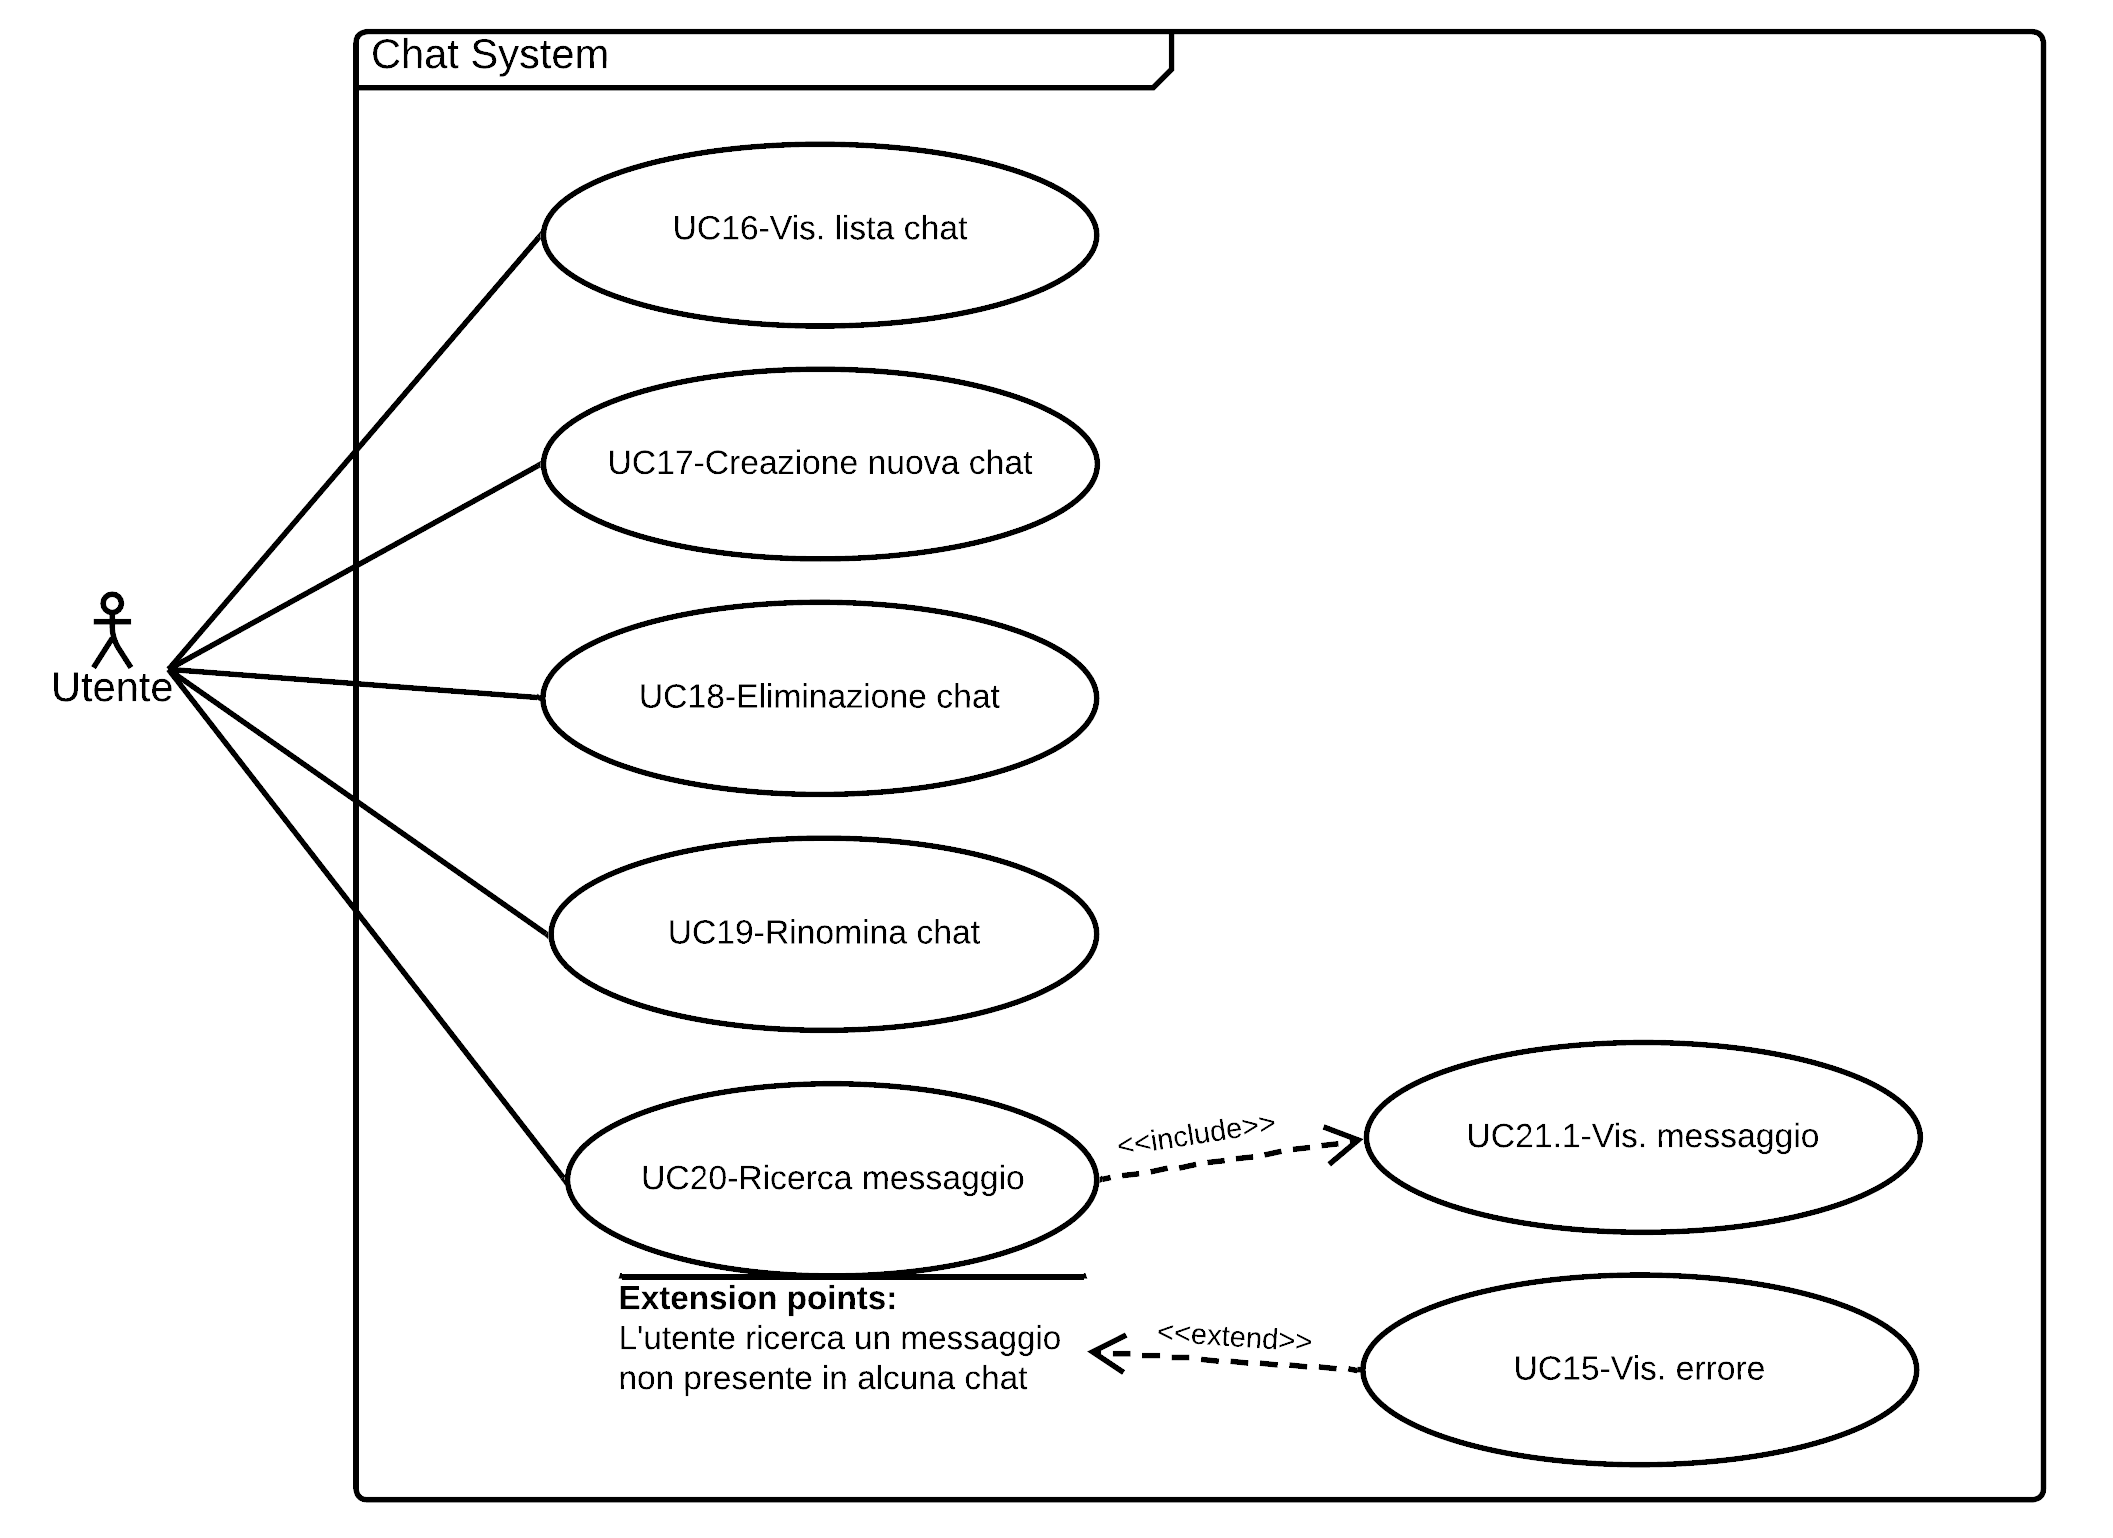
\includegraphics[width=0.75\textwidth, height=0.75\textheight, keepaspectratio]{UC-images/UC15-UC16-UC17-UC18-UC19-UC20-UC21.1.png}
        \caption{Diagramma dei Casi d'Uso UC15, UC16, UC17, UC18, UC19, UC20 e UC21.1}
    \end{figure}
    
    \subsubsection{UC16 - Visualizzazione lista chat}
    \begin{itemize}
        \item \textbf{Attore principale}: utente;
        \item \textbf{Precondizioni}: l'applicazine web è operativa e funzionante;
        \item \textbf{Postcondizioni}: 
        \begin{itemize}
            \item l'interfaccia utente è stata aggiornata per riflettere la lista delle chat presenti nel file system;
            \item l'utente è a conoscenza delle chat presenti nell'applicazione web.;
        \end{itemize}
            \item \textbf{Scenario principale}:
            \begin{enumerate}
                \item l'utente avvia l'applicazione web;
                \item l'utente visualizza la lista delle chat presenti nell'applicazione web.;
            \end{enumerate}
        \item \textbf{Trigger}: l'utente desidera visualizzare le chat presenti all'interno dell'applicazione web.
    \end{itemize}

    \begin{figure}[h]
        \centering
        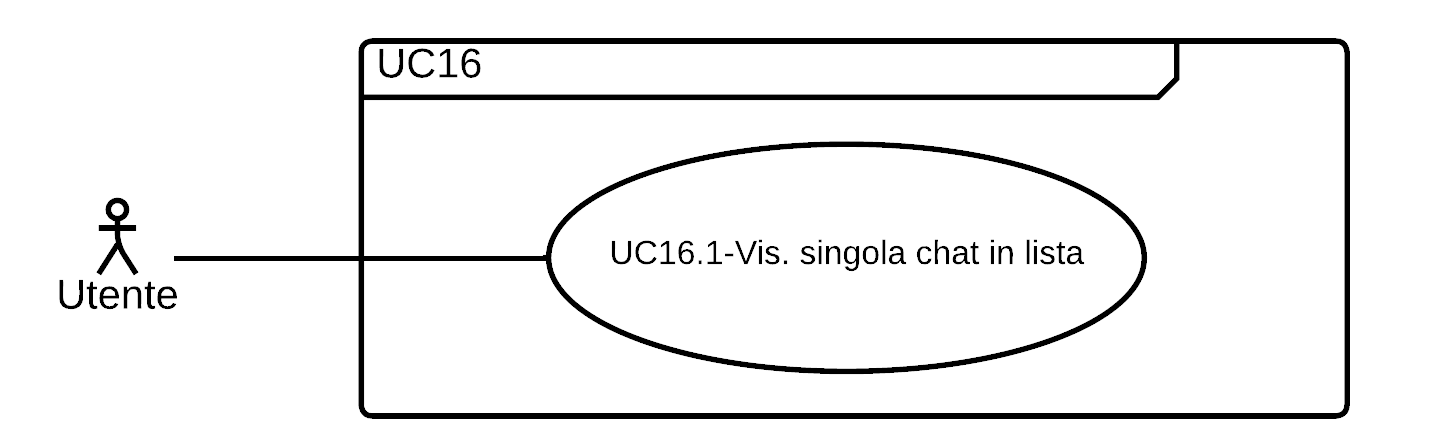
\includegraphics[width=0.75\textwidth, height=0.75\textheight, keepaspectratio]{UC-images/UC16.1.png}
        \caption{Diagramma del sotto-Caso d'Uso UC16.1}
    \end{figure}
    
    \subsubsection{UC16.1 - Visualizzazione singola chat in lista}
    \begin{itemize}
        \item \textbf{Attore principale}: utente;
        \item \textbf{Precondizioni}: 
        \begin{itemize}
            \item l'applicazine web è operativa e funzionante;
            \item l'utente ha creato almeno una chat.;
        \end{itemize}
        \item \textbf{Postcondizioni}: 
        \begin{itemize}
            \item l'interfaccia utente è stata aggiornata per riflettere la lista delle chat presenti nel file system;
            \item l'utente è a conoscenza di una particoalre chat presente nell'applicazione web.;
        \end{itemize}
        \item \textbf{Scenario principale}:
            \begin{enumerate}
                \item l'utente avvia l'applicazione web;
                \item l'utente visualizza la lista delle chat presenti nell'applicazione web.;
            \end{enumerate}
        \item \textbf{Trigger}: l'utente desidera visualizzare una chat presente all'interno della lista delle chat dell'applicazione web.
    \end{itemize}

    \begin{figure}[h]
        \centering
        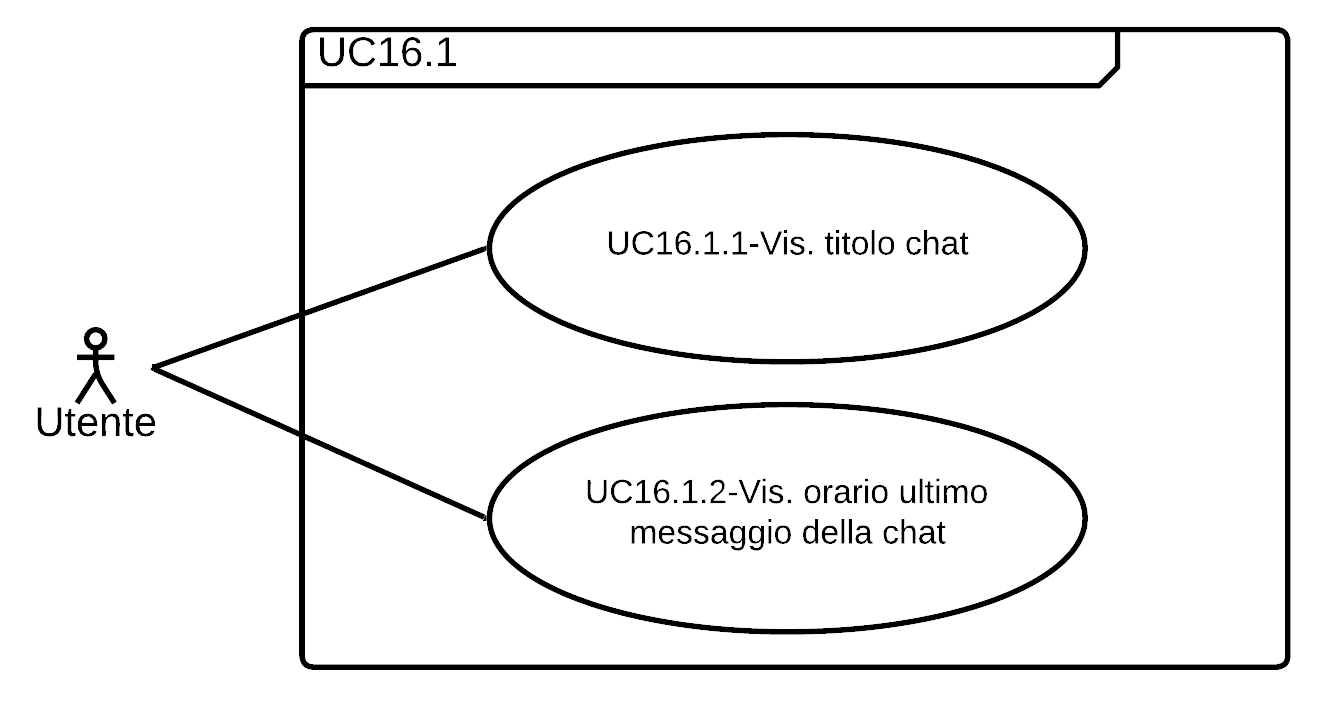
\includegraphics[width=0.75\textwidth, height=0.75\textheight, keepaspectratio]{UC-images/UC16.1.1-UC16.1.2.png}
        \caption{Diagramma dei sotto-Casi d'Uso UC16.1.1 e UC16.1.2}
    \end{figure}
    
    \subsubsection{UC16.1.1 - Visualizzazione titolo chat}
    \begin{itemize}
        \item \textbf{Attore principale}: utente;
        \item \textbf{Precondizioni}: 
        \begin{itemize}
            \item l'applicazine web è operativa e funzionante;
            \item l'utente ha creato almeno una chat.;
        \end{itemize}
        \item \textbf{Postcondizioni}: 
        \begin{itemize}
            \item l'interfaccia utente è stata aggiornata per riflettere la lista delle chat presenti nel file system;
            \item l'utente è a conoscenza del titolo di una particoalre chat presente nell'applicazione web.;
        \end{itemize}
        \item \textbf{Scenario principale}:
            \begin{enumerate}
                \item l'utente avvia l'applicazione web;
                \item l'utente visualizza la lista delle chat presenti nell'applicazione web.;
            \end{enumerate}
        \item \textbf{Trigger}: l'utente desidera visualizzare il titolo di una chat presente all'interno della lista delle chat dell'applicazione web.
    \end{itemize}

    \subsubsection{UC16.1.2 - Visualizzazione orario ultimo messaggio della chat}
    \begin{itemize}
        \item \textbf{Attore principale}: utente;
        \item \textbf{Precondizioni}: 
        \begin{itemize}
            \item l'applicazine web è operativa e funzionante;
            \item l'utente ha creato almeno una chat.;
        \end{itemize}
        \item \textbf{Postcondizioni}: 
        \begin{itemize}
            \item l'interfaccia utente è stata aggiornata per riflettere la lista delle chat presenti nel file system;
            \item l'utente è a conoscenza dell'orario dell'ultimo messaggio di una particoalre chat presente nell'applicazione web.;
        \end{itemize}
        \item \textbf{Scenario principale}:
            \begin{enumerate}
                \item l'utente avvia l'applicazione web;
                \item l'utente visualizza la lista delle chat presenti nell'applicazione web.;
            \end{enumerate}
        \item \textbf{Trigger}: l'utente desidera visualizzare l'orario dell'ultimo messaggio di una chat presente all'interno della lista delle chat dell'applicazione web.
    \end{itemize}

    \subsubsection{UC17 - Creazione nuova chat}
    \begin{itemize}
        \item \textbf{Attore principale}: utente;
        \item \textbf{Precondizioni}: l'applicazine web è operativa e funzionante;
        \item \textbf{Postcondizioni}: è stata creata una nuova chat nell'applicazione web;
        \item \textbf{Scenario principale}:
            \begin{enumerate}
                \item l'utente avvia l'applicazione web;
                \item l'utente attiva la funzionalità di creazione di una nuova chat.;
            \end{enumerate}
        \item \textbf{Trigger}: l'utente desidera creare una nuova chat all'interno dell'applicazione web.
    \end{itemize}

    \subsubsection{UC18 - Eliminazione chat}
    \begin{itemize}
        \item \textbf{Attore principale}: utente;
        \item \textbf{Precondizioni}:
        \begin{itemize}
            \item l'applicazine web è operativa e funzionante;
            \item l'utente ha creato almeno una chat.;
        \end{itemize}
        \item \textbf{Postcondizioni}: è stata eliminata chat nell'applicazione web;
        \item \textbf{Scenario principale}:
            \begin{enumerate}
                \item l'utente avvia l'applicazione web;
                \item l'utente visualizza le chat presenti nell'applicazione web (\S UC16);
                \item l'utente elimina una chat.;
            \end{enumerate}
        \item \textbf{Trigger}: l'utente desidera eliminare una chat all'interno dell'applicazione web.
    \end{itemize}

    \subsubsection{UC19 - Rinomina chat}
    \begin{itemize}
        \item \textbf{Attore principale}: utente;
        \item \textbf{Precondizioni}:
        \begin{itemize}
            \item l'applicazine web è operativa e funzionante;
            \item l'utente ha creato almeno una chat.;
        \end{itemize}
        \item \textbf{Postcondizioni}: è stata rinominata una chat nell'applicazione web;
        \item \textbf{Scenario principale}:
            \begin{enumerate}
                \item l'utente avvia l'applicazione web;
                \item l'utente visualizza le chat presenti nell'applicazione web (\S UC16);
                \item l'utente seleziona la funzionalità di rinomina della chat;
                \item l'utente fornisce un nuovo titolo alla chat;
                \item l'utente salva il titolo inserito, confermando l'operazione di rinomina.;
            \end{enumerate}
        \item \textbf{Trigger}: l'utente desidera rinominare una chat all'interno dell'applicazione web.
    \end{itemize}

    \subsubsection{UC20 - Ricerca messaggio}
    \begin{itemize}
        \item \textbf{Attore principale}: utente;
        \item \textbf{Precondizioni}:
        \begin{itemize}
            \item l'applicazine web è operativa e funzionante;
            \item l'utente ha creato almeno una chat.;
        \end{itemize}
        \item \textbf{Postcondizioni}: viene visualizzato il messaggio ricercato presente all'interno di una delle chat presenti nell'applicazione web.;
        \item \textbf{Scenario principale}:
            \begin{enumerate}
                \item l'utente avvia l'applicazione web;
                \item l'utente seleziona la funzionalità di ricerca di un messaggio tra le chat presenti nell'applicazione web;
                \item l'utente inserirsce il contenuto testuale che desidera ricercare nelle chat dell'applicazione web;
                \item l'utente attiva la ricerca del contenuto testuale;
                \item l'utente visualizza il messaggio ricercato (\S UC21.1).;
            \end{enumerate}
        \item \textbf{Scenario alternativo}: 
        \begin{enumerate}
            \item l'utente ricerca un messaggio non presente in alcuna chat nell'applicazione web;
        \end{enumerate}
        \item \textbf{Trigger}: l'utente desidera ricercare il contenuto in un messaggio all'interno dell'applicazione web.
    \end{itemize}

    \begin{figure}[h]
        \centering
        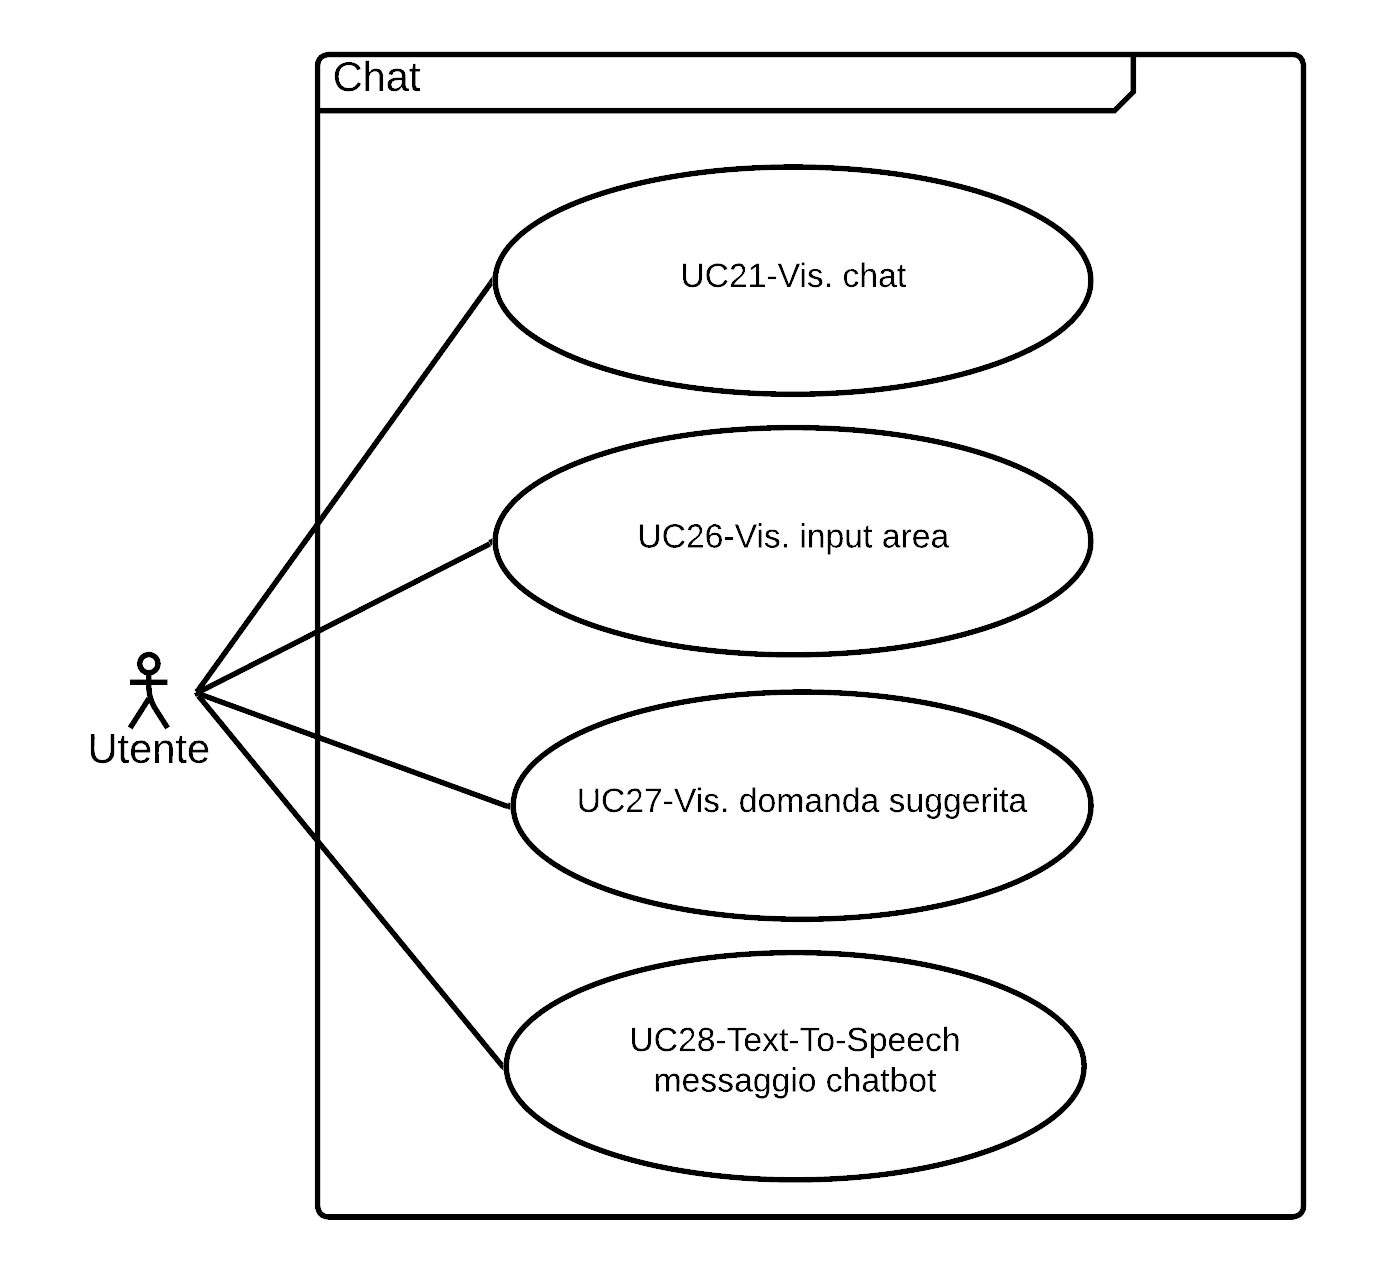
\includegraphics[width=0.75\textwidth, height=0.75\textheight, keepaspectratio]{UC-images/UC21-UC26-UC27-UC28.png}
        \caption{Diagramma dei Casi d'Uso UC21, UC26, UC27 e UC28}
    \end{figure}
    
    \subsubsection{UC21 - Visualizzazione chat}
    \begin{itemize}
        \item \textbf{Attore principale}: utente;
        \item \textbf{Precondizioni}: l'applicazine web è operativa e funzionante;
        \item \textbf{Postcondizioni}: viene visualizzata una chat presente nell'applicazione web;
        \item \textbf{Scenario principale}:
            \begin{enumerate}
                \item l'utente avvia l'applicazione web;
                \item l'utente visualizza la lista delle chat presenti nell'applicazione web (\S UC16);
                \item l'utente seleziona una chat tra quelle presenti nella lista delle chat nell'applicazione web;
                \item l'utente visualizza il contenuto della chat aperta.;
            \end{enumerate}
        \item \textbf{Trigger}: l'utente desidera visualizzare una chat tra quelle presenti all'interno dell'applicazione web.
    \end{itemize}

    \begin{figure}[h]
        \centering
        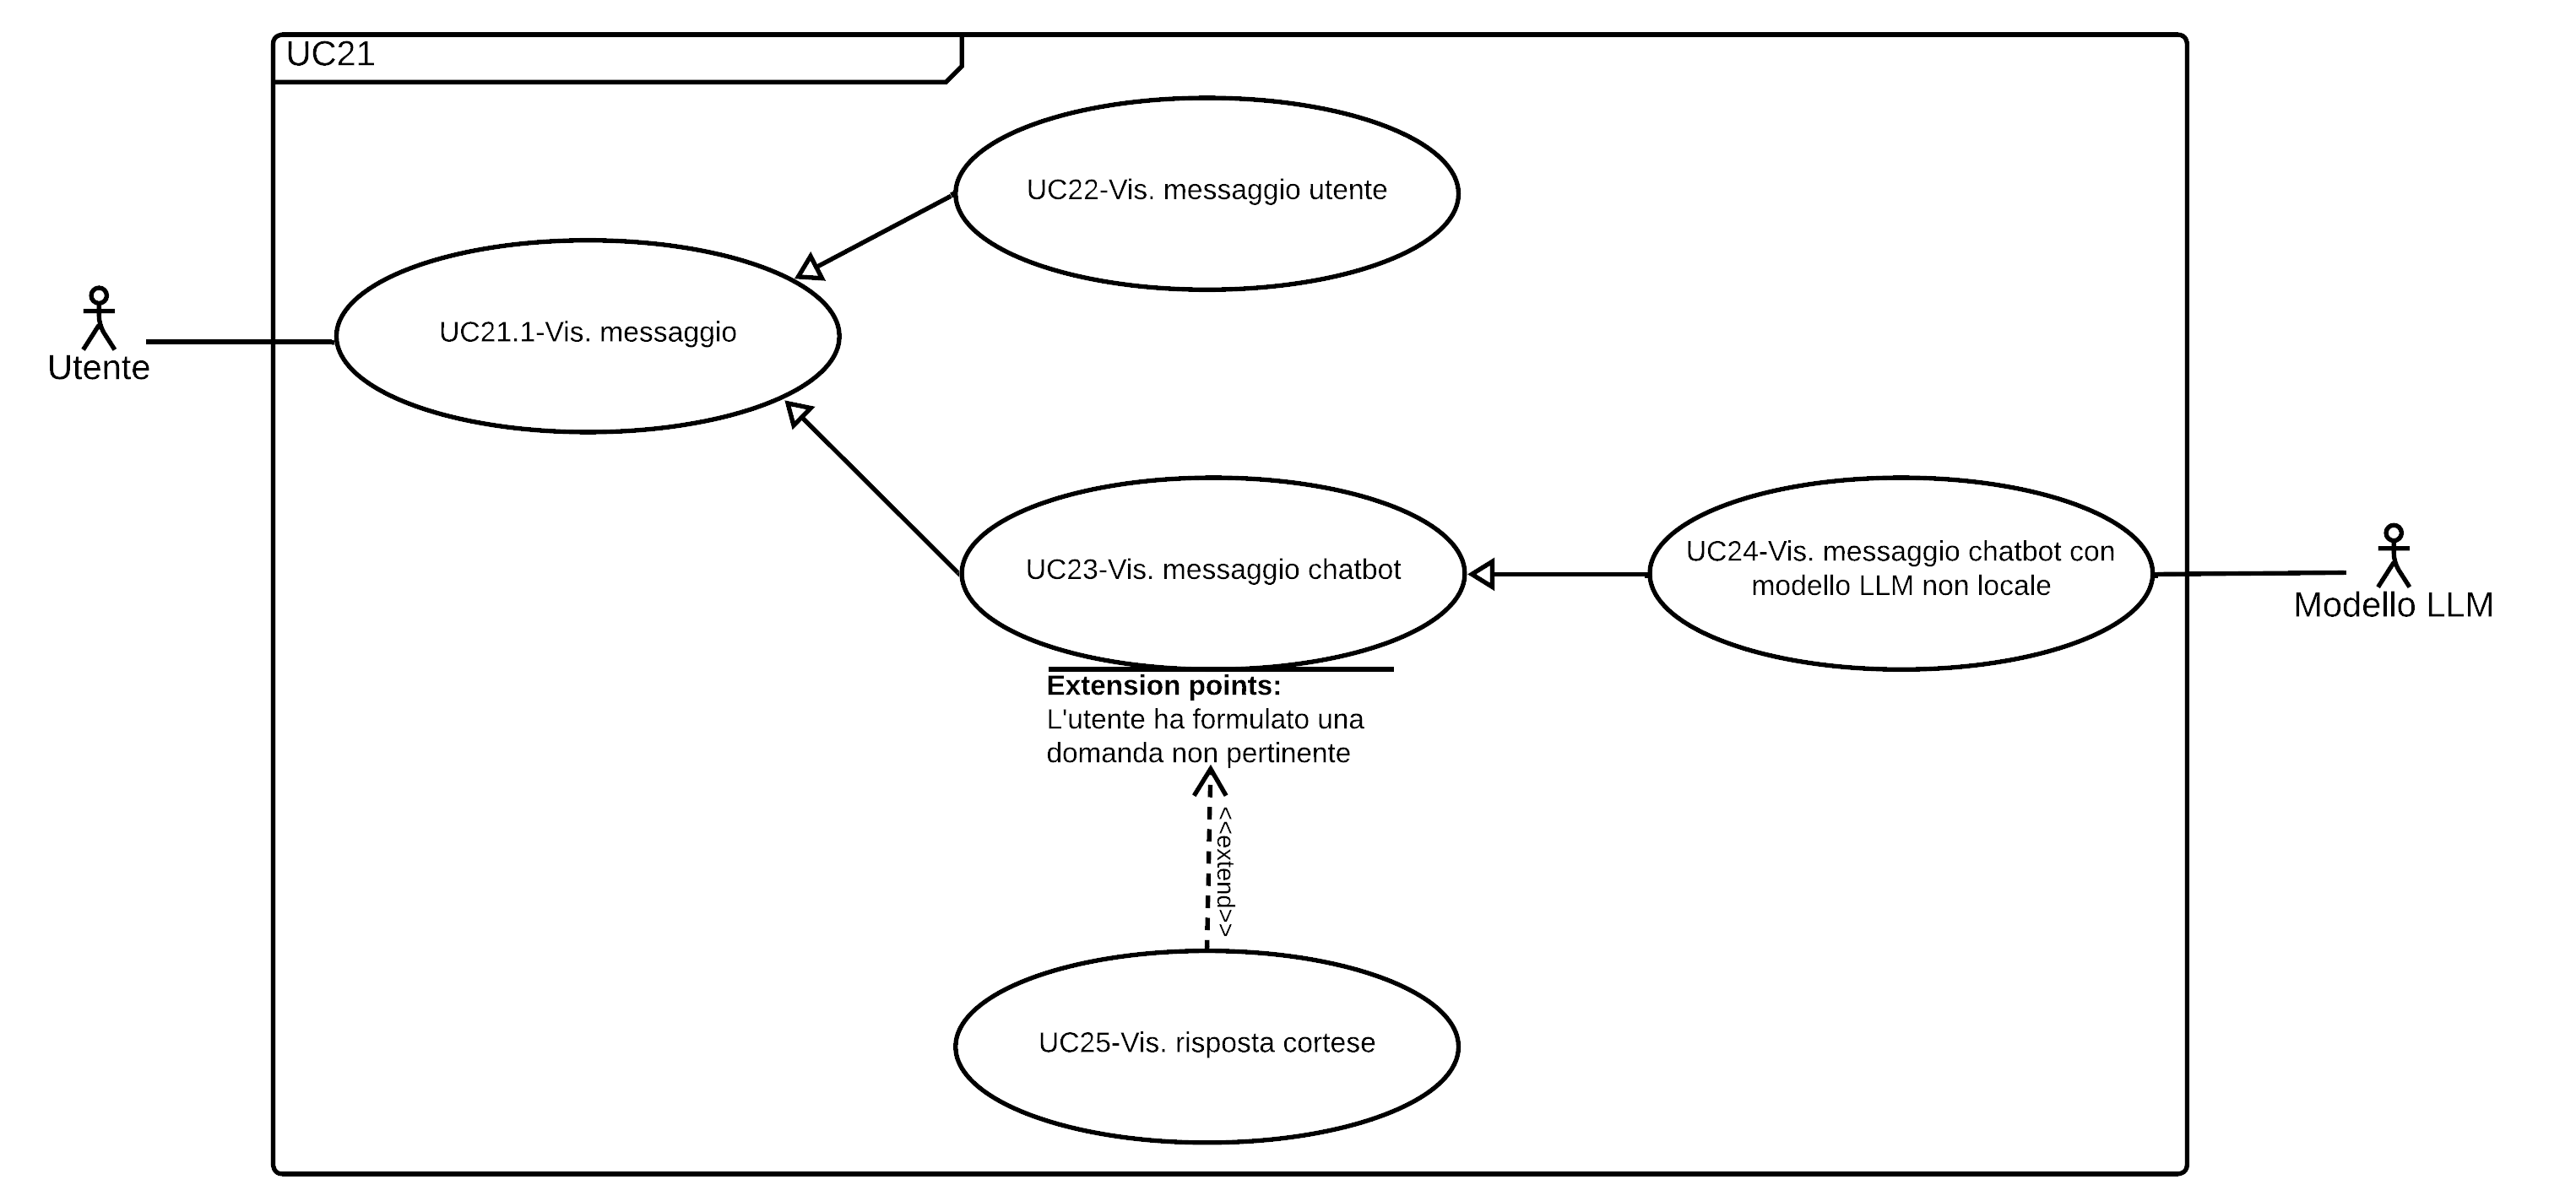
\includegraphics[width=0.75\textwidth, height=0.75\textheight, keepaspectratio]{UC-images/UC21.1-UC22-UC23-UC24-UC25.png}
        \caption{Diagramma dei Casi d'Uso UC21.1, UC22, UC23, UC24 e UC25}
    \end{figure}
    
    \subsubsection{UC21.1 - Visualizzazione messaggio}
    \begin{itemize}
        \item \textbf{Attore principale}: utente;
        \item \textbf{Precondizioni}: 
        \begin{itemize}
            \item l'applicazine web è operativa e funzionante;
            \item l'utente ha scambiato almeno un messaggio con il chatbot;
        \end{itemize}
        \item \textbf{Postcondizioni}: viene visualizzato un messaggio di una chat presente nell'applicazione web;
        \item \textbf{Scenario principale}:
            \begin{enumerate}
                \item l'utente avvia l'applicazione web;
                \item l'utente visualizza la lista delle chat presenti nell'applicazione web (\S UC16);
                \item l'utente seleziona una chat tra quelle presenti nella lista delle chat nell'applicazione web;
                \item l'utente visualizza il contenuto della chat aperta.;
            \end{enumerate}
        \item \textbf{Trigger}: l'utente desidera visualizzare un messaggio di una chat tra quelle presenti all'interno dell'applicazione web.
    \end{itemize}

    \begin{figure}[h]
        \centering
        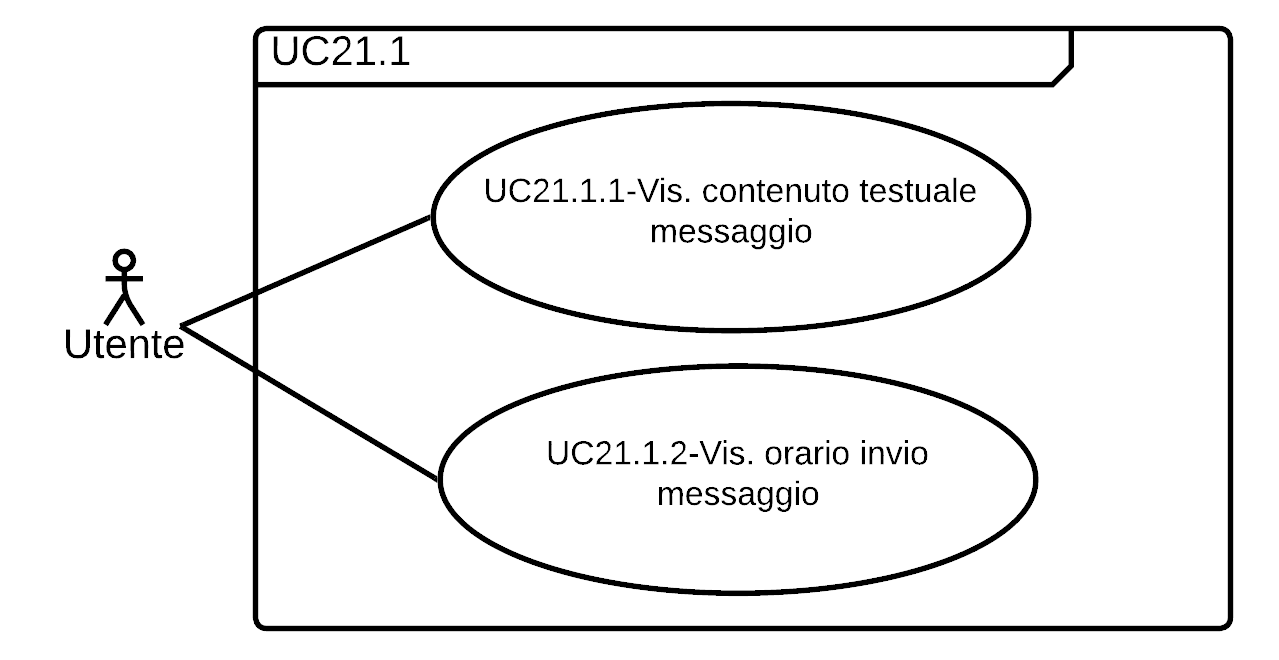
\includegraphics[width=0.75\textwidth, height=0.75\textheight, keepaspectratio]{UC-images/UC21.1.1-UC21.1.2.png}
        \caption{Diagramma dei sotto-Casi d'Uso UC21.1.1 e UC21.1.2}
    \end{figure}

    \subsubsection{UC21.1.1 - Visualizzazione contenuto testuale messaggio}
    \begin{itemize}
        \item \textbf{Attore principale}: utente;
        \item \textbf{Precondizioni}: 
        \begin{itemize}
            \item l'applicazine web è operativa e funzionante;
            \item l'utente ha scambiato almeno un messaggio con il chatbot;
        \end{itemize}
        \item \textbf{Postcondizioni}: viene visualizzato il contenuto testuale di un messaggio di una chat presente nell'applicazione web;
        \item \textbf{Scenario principale}:
            \begin{enumerate}
                \item l'utente avvia l'applicazione web;
                \item l'utente visualizza la lista delle chat presenti nell'applicazione web (\S UC16);
                \item l'utente seleziona una chat tra quelle presenti nella lista delle chat nell'applicazione web;
                \item l'utente visualizza il contenuto della chat aperta.;
            \end{enumerate}
        \item \textbf{Trigger}: l'utente desidera visualizzare il contenuto testuale di un messaggio di una chat tra quelle presenti all'interno dell'applicazione web.
    \end{itemize}

    \subsubsection{UC21.1.2 - Visualizzazione orario invio messaggio}
    \begin{itemize}
        \item \textbf{Attore principale}: utente;
        \item \textbf{Precondizioni}: 
        \begin{itemize}
            \item l'applicazine web è operativa e funzionante;
            \item l'utente ha scambiato almeno un messaggio con il chatbot;
        \end{itemize}
        \item \textbf{Postcondizioni}: viene visualizzato l'orario di invio di un messaggio di una chat presente nell'applicazione web;
        \item \textbf{Scenario principale}:
            \begin{enumerate}
                \item l'utente avvia l'applicazione web;
                \item l'utente visualizza la lista delle chat presenti nell'applicazione web (\S UC16);
                \item l'utente seleziona una chat tra quelle presenti nella lista delle chat nell'applicazione web;
                \item l'utente visualizza il contenuto della chat aperta.;
            \end{enumerate}
        \item \textbf{Trigger}: l'utente desidera visualizzare l'orario di invio di un messaggio di una chat tra quelle presenti all'interno dell'applicazione web.
    \end{itemize}
    
    \subsubsection{UC22 - Visualizzazione messaggio utente}
    \begin{itemize}
        \item \textbf{Attore principale}: utente;
        \item \textbf{Precondizioni}: 
        \begin{itemize}
            \item l'applicazine web è operativa e funzionante;
            \item l'utente ha scambiato almeno un messaggio con il chatbot;
        \end{itemize}
        \item \textbf{Postcondizioni}: viene visualizzato un messaggio scritto dall'utente di una chat presente nell'applicazione web;
        \item \textbf{Scenario principale}:
            \begin{enumerate}
                \item l'utente avvia l'applicazione web;
                \item l'utente visualizza la lista delle chat presenti nell'applicazione web (\S UC16);
                \item l'utente seleziona una chat tra quelle presenti nella lista delle chat nell'applicazione web;
                \item l'utente visualizza il contenuto della chat aperta;
                \item l'utente scrive una domanda testuale da inviare al chabot nell'area di input e formula una domanda testuale al chatbot (\S UC29) o seleziona una domanda suggerita (\S UC27);
                \item l'utente visualizza il messaggio contenente la richiesta da lui formulata.;
            \end{enumerate}
        \item \textbf{Trigger}: l'utente desidera formulare una domanda al chatbot.
    \end{itemize}

    \subsubsection{UC23 - Visualizzazione messaggio chatbot}
    \begin{itemize}
        \item \textbf{Attore principale}: utente;
        \item \textbf{Precondizioni}: 
        \begin{itemize}
            \item l'applicazine web è operativa e funzionante;
            \item l'utente ha scambiato almeno un messaggio con il chatbot;
            \item il chatbot ha fornito almeno una risposta alle richieste dell'utente.;
        \end{itemize}
        \item \textbf{Postcondizioni}: viene visualizzato un messaggio del chatbot di una chat presente nell'applicazione web;
        \item \textbf{Scenario principale}:
            \begin{enumerate}
                \item l'utente avvia l'applicazione web;
                \item l'utente visualizza la lista delle chat presenti nell'applicazione web (\S UC16);
                \item l'utente seleziona una chat tra quelle presenti nella lista delle chat nell'applicazione web;
                \item l'utente visualizza la chat selezionata;
                \item l'utente scrive una domanda testuale da inviare al chabot nell'area di input e formula una domanda testuale al chatbot (\S UC29) o seleziona una domanda suggerita (\S UC27);
                \item l'utente visualizza il messaggio contenente la richiesta da lui formulata;
                \item il chatbot fornisce una risposta alla domanda formulata dall'utente;
                \item l'utente visualizza il messaggio del chatbot.;
            \end{enumerate}
        \item \textbf{Scenario alternativo}: l'utente formula una domanda non pertinente alla documentazione sulla quale è addestrato il modello LLM utilizzato dal chatbot dell'applicazione web; 
        \item \textbf{Trigger}: l'utente ha formulato una domanda al chatbot.
    \end{itemize}

    \begin{figure}[h]
        \centering
        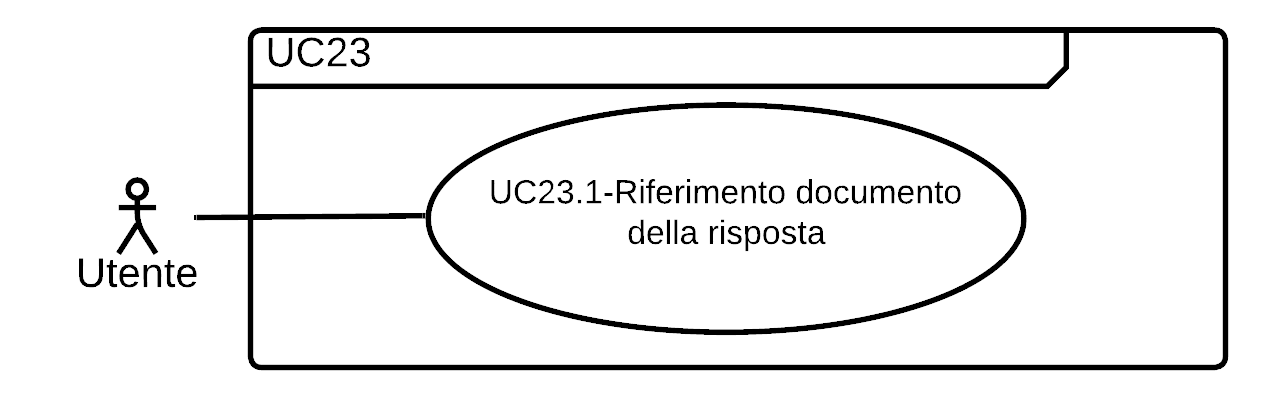
\includegraphics[width=0.75\textwidth, height=0.75\textheight, keepaspectratio]{UC-images/UC23.1.png}
        \caption{Diagramma del sotto-Caso d'Uso UC23.1}
    \end{figure}

    \subsubsection{UC23.1 - Riferimento documento della risposta}
    \begin{itemize}
        \item \textbf{Attore principale}: utente;
        \item \textbf{Precondizioni}: 
        \begin{itemize}
            \item l'applicazine web è operativa e funzionante;
            \item l'utente ha scambiato almeno un messaggio con il chatbot;
            \item il chatbot ha fornito almeno una risposta alle richieste dell'utente.;
        \end{itemize}
        \item \textbf{Postcondizioni}: il messaggio di risposta ad un messaggio utente di una chat presente nell'applicazione web presenta il riferimento al documento da cui ha estrapolato le informazioni riportate;
        \item \textbf{Scenario principale}:
            \begin{enumerate}
                \item l'utente avvia l'applicazione web;
                \item l'utente visualizza la lista delle chat presenti nell'applicazione web (\S UC16);
                \item l'utente seleziona una chat tra quelle presenti nella lista delle chat nell'applicazione web;
                \item l'utente visualizza il contenuto della chat aperta;
                \item l'utente scrive una domanda testuale da inviare al chabot nell'area di input e formula una domanda testuale al chatbot (\S UC29) o seleziona una domanda suggerita (\S UC27);
                \item l'utente visualizza il messaggio contenente la richiesta da lui formulata;
                \item il chatbot fornisce una risposta alla domanda formulata dall'utente;
                \item l'utente visualizza il messaggio del chatbot.;
            \end{enumerate}
        \item \textbf{Trigger}: l'utente ha formulato una domanda pertinente al dataset su cui il modello LLM è stato addestrato.
    \end{itemize}

    \subsubsection{UC24 - Visualizzazione messaggio chatbot con modello LLM non locale}
    \begin{itemize}
        \item \textbf{Attore principale}: utente;
        \item \textbf{Attore secondario}: modello LLM;
        \item \textbf{Precondizioni}: 
        \begin{itemize}
            \item l'applicazine web è operativa e funzionante;
            \item l'utente ha scambiato almeno un messaggio col chatbot;
            \item l'utente ha selezionato un modello LLM non locale nelle impostazioni dell'applicazione web.;
        \end{itemize}
        \item \textbf{Postcondizioni}: viene visualizzato un messaggio di risposta ad un messaggio utente di una chat presente nell'applicazione web;
        \item \textbf{Scenario principale}:
            \begin{enumerate}
                \item l'utente avvia l'applicazione web;
                \item l'utente visualizza la lista delle chat presenti nell'applicazione web (\S UC16);
                \item l'utente seleziona una chat tra quelle presenti nella lista delle chat nell'applicazione web;
                \item l'utente visualizza la chat selezionata;
                \item l'utente scrive una domanda testuale da inviare al chabot nell'area di input e formula una domanda testuale al chatbot (\S UC29) o seleziona una domanda suggerita (\S UC27);
                \item l'utente visualizza il messaggio contenente la richiesta da lui formulata;
                \item il chatbot fornisce una risposta alla domanda formulata dall'utente;
                \item l'utente visualizza il messaggio del chatbot.;
            \end{enumerate}
        \item \textbf{Scenario alternativo}: l'utente formula una domanda non pertinente alla documentazione sulla quale è addestrato il modello LLM utilizzato dal chatbot dell'applicazione web; 
        \item \textbf{Trigger}: l'utente ha formulato una domanda al chatbot.
        \end{itemize}

    \subsubsection{UC25 - Visualizzazione risposta cortese}
    \begin{itemize}
        \item \textbf{Attore principale}: utente;
        \item \textbf{Precondizioni}: 
        \begin{itemize}
            \item l'applicazine web è operativa e funzionante;
            \item l'utente ha scambiato almeno un messaggio col chatbot;
            \item l'utente ha formulato una domanda non pertinente al dataset su cui il modello LLM è stato addestrato.;
        \end{itemize}
        \item \textbf{Postcondizioni}: viene visualizzato un messaggio di risposta cortese ad un messaggio utente di una chat presente nell'applicazione web;
        \item \textbf{Scenario principale}:
            \begin{enumerate}
                \item l'utente avvia l'applicazione web;
                \item l'utente visualizza la lista delle chat presenti nell'applicazione web (\S UC16);
                \item l'utente seleziona una chat tra quelle presenti nella lista delle chat nell'applicazione web;
                \item l'utente visualizza la chat selezionata;
                \item l'utente scrive una domanda testuale non pertinente da inviare al chabot nell'area di input e formula una domanda testuale al chatbot (\S UC29);
                \item l'utente visualizza il messaggio contenente la richiesta da lui formulata;
                \item il chatbot fornisce una risposta cortese alla domanda non pertinente formulata dall'utente;
                \item l'utente visualizza il messaggio del chatbot.;
            \end{enumerate}
        \item \textbf{Trigger}: l'utente ha formulato una domanda non pertinente al dataset su cui il modello LLM è stato addestrato.
    \end{itemize}

    \subsubsection{UC26 - Visualizzazione input area}
    \begin{itemize}
        \item \textbf{Attore principale}: utente;
        \item \textbf{Precondizioni}: l'applicazine web è operativa e funzionante;
        \item \textbf{Postcondizioni}: l'utente visualizza l'area di input presente nell'applicazione web per la comunicazione con il chatbot;
        \item \textbf{Scenario principale}:
            \begin{enumerate}
                \item l'utente avvia l'applicazione web;
                \item l'utente visualizza la lista delle chat presenti nell'applicazione web (\S UC16);
                \item l'utente seleziona una chat tra quelle presenti nella lista delle chat nell'applicazione web;
                \item l'utente visualizza l'area di input presente nell'applicazione per la comunicazine con il chatbot.;
            \end{enumerate}
        \item \textbf{Trigger}: l'utente desidera visualizzare l'area di input presente nell'applicazione web per la comunicazione con il chatbot.
    \end{itemize}

    \subsubsection{UC27 - Visualizzazione domanda suggerita}
    \begin{itemize}
        \item \textbf{Attore principale}: utente;
        \item \textbf{Precondizioni}: l'applicazine web è operativa e funzionante;
        \item \textbf{Postcondizioni}: nell'area di testo dell'input area è ora presente la domanda testuale suggerita all'utente;
        \item \textbf{Scenario principale}:
            \begin{enumerate}
                \item l'utente avvia l'applicazione web;
                \item l'utente visualizza la lista delle chat presenti nell'applicazione web (\S UC16);
                \item l'utente apre una chat tra quelle presenti nella lista delle chat nell'applicazione web;
                \item l'utente visualizza la domanda suggerita nella chat.;
            \end{enumerate}
        \item \textbf{Trigger}: l'utente desidera formualare una domanda al chatbot.
    \end{itemize}

    \subsubsection{UC28 - Text-To-Speech messaggio chatbot}
    \begin{itemize}
        \item \textbf{Attore principale}: utente;
        \item \textbf{Precondizioni}: 
        \begin{itemize}
            \item l'applicazine web è operativa e funzionante;
            \item il chatbot ha elaborato un messaggio di risposta ad un messaggio dell'utente;
            \item l'utente ha selezionato la funzionalità Text-To-Speech.;
        \end{itemize}
        \item \textbf{Postcondizioni}: il messaggio desiderato è stato letto dal sistema all'utente;
        \item \textbf{Scenario principale}:
            \begin{enumerate}
                \item l'utente avvia l'applicazione web;
                \item l'utente visualizza la lista delle chat presenti nell'applicazione web (\S UC16);
                \item l'utente seleziona una chat tra quelle presenti nella lista delle chat nell'applicazione web;
                \item l'utente scrive una domanda testuale da inviare al chabot nell'area di input e formula una domanda testuale al chatbot (\S UC29) o seleziona una domanda suggerita (\S UC27);
                \item l'utente visualizza il messaggio contenente la richiesta da lui formulata;
                \item il chatbot fornisce una risposta alla richiesta dell'utente;
                \item l'utente visualizza il messaggio del chatbot;
                \item l'utente seleziona la funzionalità Text-To-Speech.;
                \item l'utente ascolta la lettura del messaggio del chatbot.;
            \end{enumerate}
        \item \textbf{Trigger}: l'utente attiva la funzionalità Text-To-Speech su un messaggio del chatbot.
    \end{itemize}

    \begin{figure}[h]
        \centering
        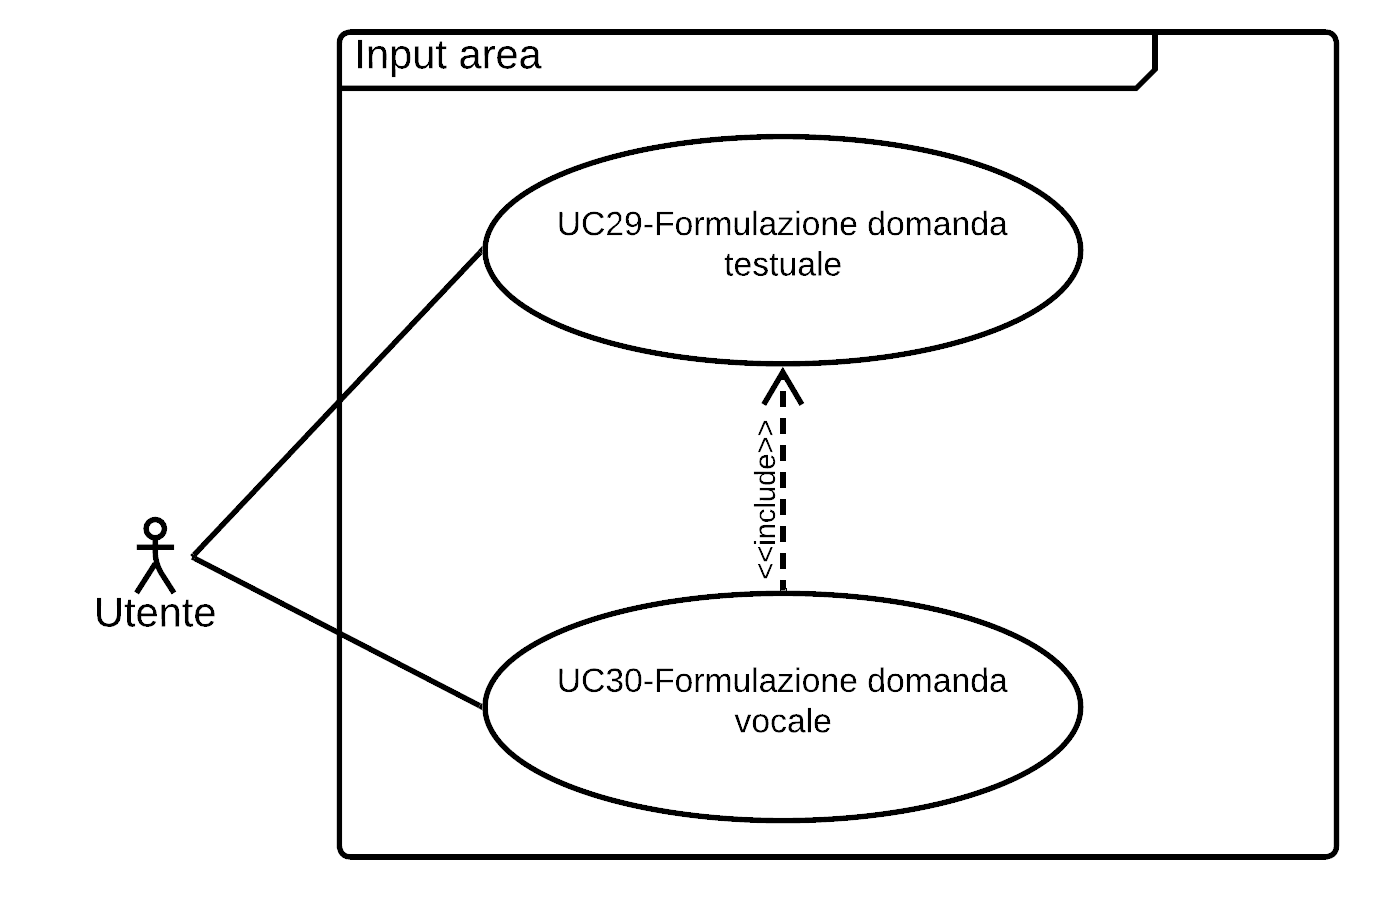
\includegraphics[width=0.75\textwidth, height=0.75\textheight, keepaspectratio]{UC-images/UC29-UC30.png}
        \caption{Diagramma dei Casi d'Uso UC29 e UC30}
    \end{figure}

    \subsubsection{UC29 - Formulazione domanda testuale}
    \begin{itemize}
        \item \textbf{Attore principale}: utente;
        \item \textbf{Precondizioni}: l'applicazine web è operativa e funzionante;
        \item \textbf{Postcondizioni}: l'utente ha formualto una domanda testuale al chatbot;
        \item \textbf{Scenario principale}:
            \begin{enumerate}
                \item l'utente avvia l'applicazione web;
                \item l'utente visualizza la lista delle chat presenti nell'applicazione web (\S UC16);
                \item l'utente seleziona una chat tra quelle presenti nella lista delle chat nell'applicazione web;
                \item l'utente visualizza l'area di input presente nell'applicazione per la comunicazine con il chatbot;
                \item l'utente scrive una domanda testuale nell'area di input;
                \item l'utente invia la domanda testuale al chatbot.;
            \end{enumerate}
        \item \textbf{Trigger}: l'utente desidera formualare una domanda al chatbot.
    \end{itemize}

    \subsubsection{UC30 - Formulazione domanda vocale}
    \begin{itemize}
        \item \textbf{Attore principale}: utente;
        \item \textbf{Precondizioni}: l'applicazine web è operativa e funzionante;
        \item \textbf{Postcondizioni}: nell'area di testo dell'input area è ora presente la domanda testuale formulata dall'utente;
        \item \textbf{Scenario principale}:
            \begin{enumerate}
                \item l'utente avvia l'applicazione web;
                \item l'utente visualizza la lista delle chat presenti nell'applicazione web (\S UC14);
                \item l'utente apre una chat tra quelle presenti nella lista delle chat nell'applicazione web;
                \item l'utente visualizza l'area di input presente nell'applicazione per la comunicazine con il chatbot;
                \item l'utente attiva la funzionalità vocale;
                \item l'utente formula oralmente la domanda da sottoporre al chatbot;
                \item la domanda vocale viene tradotta in domanda testuale.;
            \end{enumerate}
        \item \textbf{Trigger}: l'utente desidera formualare una domanda vocale al chatbot.
    \end{itemize}

%\renewcommand{\arraystretch}{1.5}
%\begin{tabularx}{\textwidth}{|c|X|c|c|c|}\hline
%\textbf{Caso d'uso} & \textbf{Attori} & \textbf{Precondizioni} & %\textbf{Postcondizioni} & \textbf{Scenario principale} \\
%\end{tabularx}


% REQUISITI
\newpage

\section{Requisiti}
Ogni requisito preso in analisi sarà trattato con la sigla:\\
R[Tipo].[Importanza].[Ordine];\\
nella quale:\\
\begin{itemize}
\item R indica la parola "requisito";
\item Tipo può essere:
    \begin{itemize}
	\item F (Funzionale);
	\item Q (Qualità);
	\item V (Vincolo).
    \end{itemize}
\item Importanza può essere:
    \begin{itemize}
        \item O (Obbligatorio);
	\item D (Desiderabile);
	\item OP (Opzionale).
    \end{itemize}
\item Ordine: indica l’ordine in cui il requisito è stato preso in esame. Per i requisiti con stessa importanza e tipologia indica l’ordine cronologico di precedenza che esso ha avuto rispetto agli altri, ovvero il suo ordine inserimento nell'Analisi dei requisiti.
\end{itemize}
N.B: per requisiti che dovessero generare requisiti figli, si andrà ad aggiungere .[N.figlio] alla notazione successivamente all’ordine, di modo da avere i figli ordinati per importanza.

\subsection{Requisiti funzionali}
Di seguito la specifica per i requisiti funzionali, i quali descrivono le funzionalità del sistema, le azioni
che il sistema può compiere e le informazioni che il sistema può fornire.
Le sigle sotto riportate indicano:
\begin{itemize}
    \item ROF - Requisito Obbligatorio Funzionale;
    \item RDF - Requisito Desiderabile Funzionale;
    \item ROPF - Requisito Opzionale Funzionale.
\end{itemize}

\renewcommand{\arraystretch}{1.5}
\begin{xltabular}{\textwidth}{|c|X|c|c}\hline
\textbf{Codice} & \textbf{Descrizione}  & \textbf{Fonti} \\
\hline ROF1\ & L'utente deve poter accedere all'applicazione web. &  UC1 \\
\hline ROF2\ & L'utente deve poter visualizzare i modelli LLM resi disponibili nell'applicazione per il chatbot. & UC2 \\
\hline ROF2.1\ & L'utente deve poter visualizzare il nome dei modelli LLM resi a disposizione nell'applicazione web. & UC2.1.1 \\
\hline ROF2.2\ & L'utente deve poter visualizzare l'organizzazione che offre un modello LLM reso a disposizione nell'applicazione web. & UC2.1.2 \\
\hline ROF2.3\ & L'utente deve poter visualizzare le caratteristiche dei modelli LLM resi a disposizione nell'applicazione web. & UC2.1.3 \\
\hline ROF3\ & L'utente deve poter configurare il modello LLM utilizzato dal chatbot. & UC3 \\
\hline ROF4\ & L'utente deve poter visualizzare i vector DB resi disponibili nell'applicazione web. & UC4 \\
\hline ROF4.1\ & L'utente deve poter visualizzare il nome dei vector DB resi a disposizione nell'applicazione web. & UC4.1.1 \\
\hline ROF4.2\ & L'utente deve poter visualizzare l'organizzazione che offre un vector DB reso a disposizione nell'applicazione web. & UC4.1.2 \\
\hline ROF4.3\ & L'utente deve poter visualizzare le caratteristiche dei vector DB resi a disposizione nell'applicazione web. & UC4.1.3 \\
\hline ROF5\ & L'utente deve poter configurare il vector DB utilizzato dall'applicazione web. & UC3 \\
\hline ROF6\ & L'utente deve poter visualizzare le modalità di archiviazione dei documenti rese disponibili nell'applicazione web. & UC6 \\
\hline ROF6.1\ & L'utente deve poter visualizzare il nome della modalità di archiviazione dei documenti resa a disposizione nell'applicazione web. & UC6.1.1 \\
\hline ROF6.2\ & L'utente deve poter visualizzare le caratteristiche della modalità di archiviazione dei documenti resa a disposizione nell'applicazione web. & UC6.1.2 \\
\hline ROF7\ & L'utente deve poter configurare la modalità di archiviazione utilizzata dall'applicazione web. & UC3 \\
\hline ROF8\ & L'utente deve poter visualizzare i documenti presenti nell'applicazione web. & UC8 \\
\hline ROF8.1\ & L'utente deve poter visualizzare i nomi dei documenti presenti nell'applicazione web. & UC8.1.1 \\
\hline RDF8.2\ & L'utente deve poter visualizzare le dimensioni dei documenti presenti nell'applicazione web. & UC8.1.2 \\
\hline RDF8.3\ & L'utente deve poter visualizzare se i documenti presenti nell'applicazione web appartengono al dataset di addestramento del modello LLM. & UC8.1.3 \\
\hline ROF9\ & L'utente deve poter caricare un documento di tipo .pdf. & UC9, UC9.1\\
\hline RDF9.1\ & L'utente deve poter caricare più documenti di tipo .pdf. & UC9, UC9.1, UC10 \\
\hline RDF10\ & L'utente deve poter caricare un documento di tipo .docx. & UC9, UC9.2 \\
\hline RDF10.1\ & L'utente deve poter caricare uno o più documenti di tipo .docx. & UC9, UC9.2, UC10 \\
\hline ROPF11\ & L'utente deve visualizzare un errore nel caso in cui carichi un documento vuoto. & UC9, UC10, UC15 \\
\hline ROF12\ & L'utente deve visualizzare un errore nel caso in cui carichi un documento non supportato. & UC9, UC10, UC15 \\
\hline RDF13\ & L'utente deve visualizzare un errore nel caso in cui carichi un documento già presente nel filesystem. & UC9, UC10, UC15 \\
\hline ROF14\ & L'utente deve poter aprire un documento presente nell'applicazione web. & UC8, UC11 \\
\hline ROF15\ & L'utente deve poter eliminare un documento presenti nell'applicazione web. & UC12\\
\hline ROF16.1\ & L'utente deve poter eliminare più documenti presenti nell'applicazione web. & UC13\\
\hline ROF17\ & L'utente deve poter avviare l'addestrameto del modello LLM. & UC14 \\
\hline ROF18\ & Il modello LLM deve essere addestrato con i documenti presenti nell'applicazione web. & UC14 \\
\hline ROF19\ & L'utente deve poter visualizzare tutte le chat aperte nell'applicazione. & UC16 \\
\hline ROF19.1\ & L'utente deve poter visualizzare il titolo di tutte le chat aperte nell'applicazione. & UC16.1.1 \\
\hline RDF19.2\ & L'utente deve poter visualizzare l'orario dell'ultimo messaggio di tutte le chat aperte nell'applicazione. & UC16.1.2 \\
\hline ROF20\ & L'utente deve poter creare una nuova chat. & UC17 \\
\hline ROF21\ & L'utente deve poter eliminare una chat. & UC18 \\
\hline RDF22\ & L'utente deve poter rinominare una chat. & UC19 \\
\hline ROPF23\ & L'utente deve poter ricercare un messaggio. & UC20 \\
\hline ROF24\ & L'utente deve poter visualizzare il contenuto di una chat. & UC21 \\
\hline ROF24.1\ & L'utente deve poter visualizzare un messaggio presente in una chat. & UC21.1 \\
\hline ROF24.1.1\ & L'utente deve poter visualizzare il contenuto testuale di un messaggio presente in una chat. & UC21.1.1 \\
\hline ROF24.1.2\ & L'utente deve poter visualizzare l'orario di invio di un messaggio presente in una chat. & UC21.1.2 \\
\hline ROF25\ & L'utente deve poter visualizzare un messaggio da lui inviato. & UC21, UC22, UC29 \\
\hline ROF26\ & Il chatbot deve rispondere al messaggio inviato da un utente. & UC21, UC23 \\
\hline RDF26.1\ & La risposta fornita dal chatbot deve presentare un riferimento al documento da cui ha estrapolato le informazioni esposte. & UC21, UC23, UC23.1 \\
\hline ROF27\ & L'utente deve poter visualizzare l'area di input. & UC26 \\
\hline RDF28\ & L'utente deve poter visualizzare una domanda suggerita da porre al chatbot. & UC34 \\
\hline RDF29\ & L'utente deve poter selezionare una domanda suggerita per porla al chatbot. & UC34, UC29 \\
\hline ROPF30\ & L'utente deve poter ascoltare tramite audio la risposta fornita dal chatbot (Text-To-Speech). & UC20, UC23, UC28 \\ 
\hline ROF31\ & L'utente deve poter formulare una domanda testuale al chatbot. & UC29 \\
\hline ROF32\ & L'utente deve poter formulare oralmente una domanda al chatbot. & UC30 \\
\hline
\end{xltabular}

\subsection{Requisiti di qualità}
Di seguito la specifica per i requisiti di qualità, i quali descrivono come un sistema deve essere, o
come il sistema deve esibirsi, per soddisfare le esigenze dell'utente.
Le sigle sotto riportate possono essere così classificate:
\begin{itemize}
    \item ROQ - Requisito Obbligatorio di Qualità;
    \item RDQ - Requisito Desiderabile di Qualità;
    \item ROPQ - Requisito Opzionale di Qualità.
\end{itemize}
\renewcommand{\arraystretch}{1.5}
\begin{tabularx}{\textwidth}{|c|X|c|c}\hline
\textbf{Codice} & \textbf{Descrizione}  & \textbf{Fonti} \\
\hline ROQ1 & Il sistema deve garantire il servizio per almeno un utente. & Verbale Esterno 2023-11-15 \\
\hline ROQ2 & Le chat devono essere salvate in automatico. & Verbale Esterno 2023-11-24 \\
\hline ROQ3 & L'applicazione web deve garantire la presenza di almeno un modello AI locale. & Verbale Esterno 2023-11-22 \\
\hline RDQ4 & L'applicazione in caso di caduta dalle connessione va in fallback su un modello AI locale. & Verbale Esterno 2023-11-22 \\
\hline ROQ5 & Il chatbot, in caso l'utente formuli una richiesta non pertinente al dataset di addestramento, deve fornire una risposta cortese in cui espone la sua incapacità nel fornire una risposta alla domanda. & UC20, UC22, UC24 \\ 
\hline RDQ6 & Il chatbot deve presentare la funzionalità \textit{Cache}: se l'utente formula più volte la stessa domanda il chatbot fornisce la risposta elaborata alla prima occorrenza della domanda. & Verbale Esterno 2023-11-29 \\
\hline RDQ7 & L'eliminazione di un documento deve effettuare l'eliminazione dei metadati del relativo documento, ma non all'eliminazione degli emmbeddings generati dallo stesso. & Verbale Esterno 2023-11-24 \\
\hline
\end{tabularx}

\subsection{Requisiti di vincolo}
Di seguito la specifica per i requisiti di vincolo, i quali descrivono i limiti e le restrizioni normative/legislative che un sistema
deve rispettare per soddisfare le esigenze dell'utente.
Le sigle sotto riportate possono essere così classificate:
\begin{itemize}
    \item ROV - Requisito Obbligatorio di Vincolo;
    \item RDV - Requisito Desiderabile di Vincolo;
    \item ROPV - Requisito Opzionale di Vincolo. 
\end{itemize}
\renewcommand{\arraystretch}{1.5}
\begin{tabularx}{\textwidth}{|c|X|c|c}\hline
\textbf{Codice} & \textbf{Descrizione} & \textbf{Fonti} \\
\hline
ROV1 & Il sistema deve offrire opzioni che garantiscono la privacy delle informazioni sensibili condivise dall'utente per l'addestramento del modello. & - \\
\hline

\end{tabularx}




\end{document}
